\chapter{Реализация модульной платформы технологического оборудования}\label{ch:ch4}

\section{Общие положения}

Модульная технологическая платформа (сокр. \textit{МТП}) представляет собой прототип оборудования, спроектированный и разработанный на основе рассмотренных в предыдущих главах методик. Основа МТП "--- универсальное шасси (сокр. \textit{УШ}), которое осуществляет перемещение каретки с подвесом, на который устанавливаются унифицированные модули, определяющие операции, реализуемые конкретной конфигурацией МТП. В соответствии с  методикой информационного взаимодействия УШ и каждый модуль является автономным и обладает своим собственным блоком управления и блоком коммуникации.

В соответствии с методикой проектирования МТП является \textit{унифицированной} и \textit{гибридизирванной}. Как уже отмечалось ранее, под унификацией понимаются выделение базового агрегата и совместимых с ним по конструктивным параметрам модулей. Таким образом, новая конфигурация оборудования создается как совокупность модулей, собираемых по принципу детского конструктора, то есть без необходимости выполнять какие-то дополнительные действия по механической выверке при установки модуля, либо производить настройку программного обеспечения системы ЧПУ. На рисунке представлены различные виды оборудования, которые могут быть реализованы заменой модулей в МТП, здесь видно, что несмотря на то, что все представленные образцы оборудования относятся к разным классам и имеют разных производителей, прослеживается явная общность их конструкции. На определенной координатной платформе, осуществляющей перемещение некоторого подвеса (каретки) в пространстве, размещён рабочий орган, реализующий ту или иную операцию по обработке или контролю объекта. При этом все представленные образцы оборудования имеют примерно одинаковые размеры, массу и класс точности. Последнее ещё раз подтверждает подтверждает необходимость унификации подобных видов оборудования в рамках МТП.

\begin{figure}[ht]
	\centerfloat{
		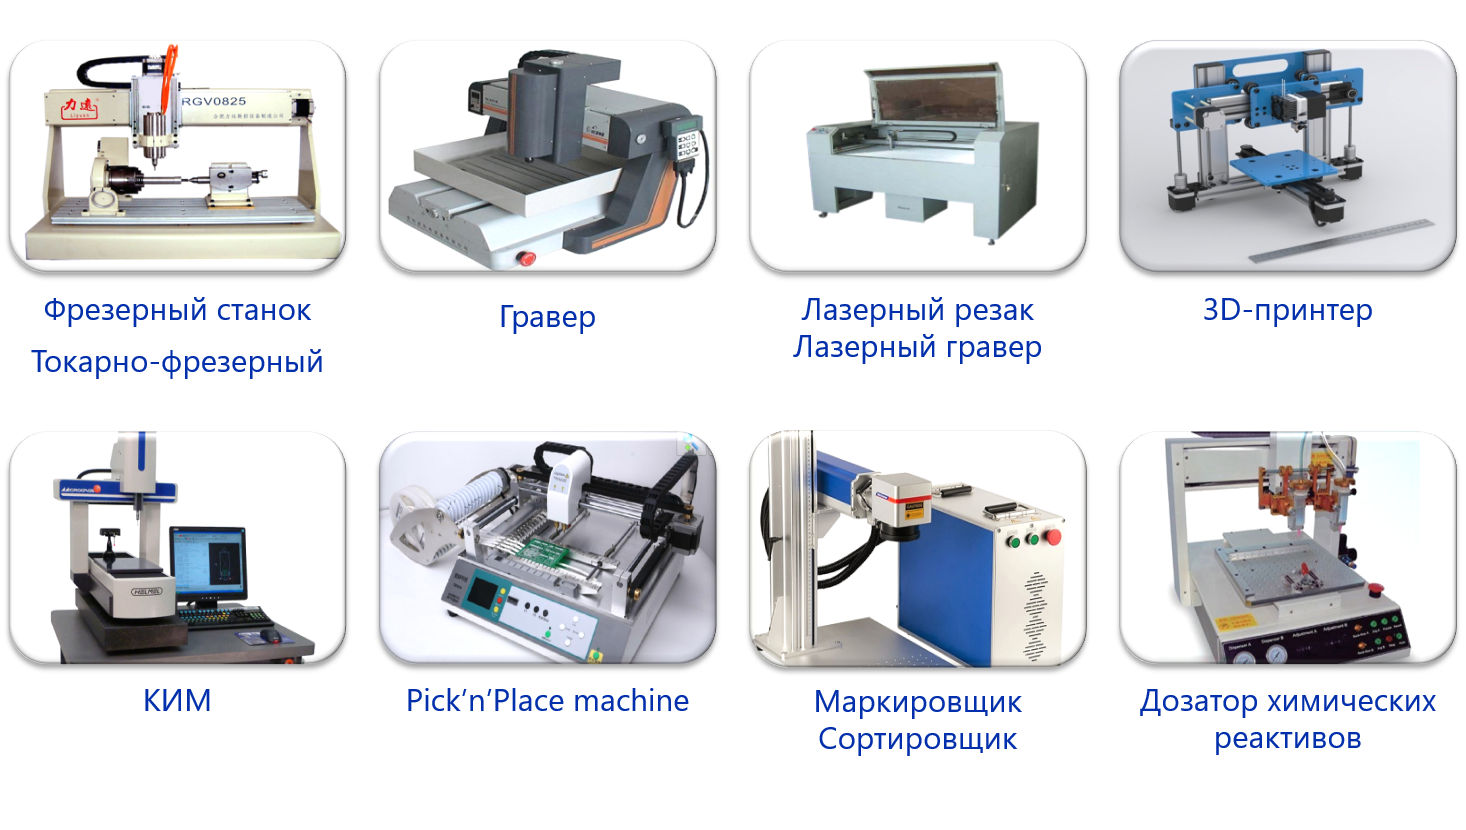
\includegraphics[width=\textwidth]{ch-4/equip-types}
	}
	\caption{Оборудование, которое можно создать на базе МТП (КИМ "--- координатно-измерительная машина).}\label{fig:equip-types}
\end{figure}

Гибридизация возможна за счет наличия параметрического ряда шасси и модулей. В зависимости от используемого типоразмера на каретке подвеса может быть закреплено несколько модулей одновременно. Таким образом, может быть реализована последовательность операций, выполняемых без переустанова объекта обработки (измерения). В эту же последовательность могут быть включены операции контроля, которые могут быть реализованы за счет установки, например, специализированного модуля машинного зрения. За счёт этого не только сокращается время подготовительно-заключительных операций, но и повышается точность обработки, уменьшается количество брака.

Например, может быть создана установка на подвесе которой установлен модуль трёхмерной печати, совмещенный со сверлильным модулем. Такая установка при соответствующей конструкции обрабатываемой заготовки может реализовать комбинированный технологический процесс, включающий в себя операцию послойного наплавления методом экструдирования расплавленного термопласта, с последующей калибровкой установочных отверстий за один установ. Также можно создать комбинированное оборудование, позволяющее дозировать паяльную пасту на печатной плате с последующей установкой на ней радиоэлектронных компонентов. Также есть возможность комбинировать любые обрабатывающие модули с лазерным модулем для гравировки/маркировки готовых изделий. 


\section{Практическая применимость модульной технологической платформы}

Как показывает практика в последние десятилетия в России появляется все больше и больше производственных компаний, которые занимаются научно-исследовательскими и опытно-конструкторскими работами для государственных и частных заказчиков. Как уже отмечалось ранее подобного рода компании получили название малые инновационные предприятия (сокр. \textit{МИП}) или стартапами\footnote{От англ. \textit{startup company, startup}, букв. <<стартующий>>.} В силу своей специфика МИП как правило занимаются проектированием и разработкой наукоёмкой продукции. Причём серийность подобного производства невысока, как правило выпускаются единичные экземпляры, либо мелкие серии. Задача МИП проработать в <<железе>> некоторую концепцию для максимально быстрого вывода нового высокотехнологичного продукта на рынок (что даст компании конкурентные преимущества), либо демонстрации работающего прототипа инвестору для организации в дальнейшем крупного производства. Также не стоит забывать о том, что МИП могут участвовать в различных научных разработках, финансируемых государством, либо частными компаниями. Подобные научно-исследовательские имеют ограниченный срок разработки, результатом которой должен стать опытный образец какого-либо изделия.

Для реализации подобных проектов МИП должны обладать парком оборудования, дающего возможность выполнять разнообразные технологические операции: от механической обработки изделий и создания радиоэлектронных компонентов до автоматизированного контроля в процессе производства, а также на этапе выпуска готовой продукции. Однако большинство МИП не в состоянии обеспечить себя всем необходимым оборудованием и поэтому вынуждены заниматься только разработкой конструкторской документации, передавая производство другим компаниям, обозначаемым термином ОЕМ~(от англ. \textit{Original Equipment Manufacturer}). Принимая во внимание все вышесказанное, необходимо отметить, что такой подход обладает рядом существенных недостатков:

\begin{enumerate}
	\item OEM являются как правило узкоспециализированными, то есть выполняют заказы на изготовление только отдельных компонентов изделий. Например, это может быть изготовление печатных плат, литье корпусных изделий из пластмасс, механическая обработка. Безусловно, существуют и крупные OEM компании, которые реализуют полный цикл производства продукции, но такие компании также ориентированы на выпуск однотипных изделий, под которые у них есть необходимое оборудование, специалисты и материалы. Например, это может быть компания по выпуску мобильных телефонов или компьютерных комплектующих, которые принимают заказы на изготовление именно такой продукции, с максимальным количеством стандартных компонентов и с учетом производственных возможностей, которыми они обладают.
	\item OEM компании в основном заинтересованы в крупных заказах, т.\,к. для них смена номенклатуры связана с необходимостью каждый раз перестраивать весь производственный процесс. Соответственно, существенная часть времени уходит на технологическую подготовку производства, что значительно повышает себестоимость единицы продукции при работе с малыми партиями. 
	\item OEM-компании работают только с заказами, которые могут выполнить максимально быстро и просто на том оборудовании и с учётом тех технологий, которые у них отлажены. Также OEM-компании работают с определенными поставщиками комплектующих, поэтому проектировщики в достаточной мере ограничены и должны учитывать специфику производства той OEM-компании, в которую они планируют обратиться.
	\item работа с OEM компаниями увеличивает время вывода на рынок новых видов продукции. Это может быть связано со множеством факторов таких, как необходимость заключения договора на производство и его юридического сопровождения, необходимость согласования конструкторской и технологической документации, передаваемой OEM компании, перегруженность производства OEM компании, необходимость изменения конструкции изделия исходя из возможностей производства и т.\,д.
	\item Всегда существует риск потери интеллектуальной собственности, связанный с передачей полного комплекта документации на выпускаемые изделия. Так как МИП занимаются разработкой наукоёмкой продукции, которая к тому же зачастую выпускается в рамках выполнения договоров на научно-исследовательские работы, заказчиком которых является государство, передача документов сторонним компаниям может быть невозможна в принципе.
	\item OEM компании занимаются только производством по готовой документации, соответственно вопрос создания быстрых прототипов изделий, предсерийных образцов и установочных партий изделий для МИП остается нерешенным.
\end{enumerate}


Другим вариантом изготовления продукции для МИП является работа с т.\,н. инжиниринговыми центрами, то есть с производственными организациями, оказывающие услуги по подготовке и обеспечению производственного процесса и всего, что с ним связано. Как правило, инжиниринговый центры строятся на базе существующих предприятий учебных/научных заведений с имеющейся базой современного технологического оборудования. В рамках работы инжиниринговых центров задействуются ресурсы, которые не участвуют (участвуют частично) в основной деятельности предприятия/организации, на базе которой существует инжиниринговый центр. Подход к производству, предполагающий, что МИП будут сотрдничать с одним или несколькими инжиниринговыми центрами в целом похож на предыдущий. Однако есть несколько различий. Во-первых, проект дробится и для каждой составной части будущего изделия подбирается соответствующий исполнитель, а также определяется форма взаимодействия с ним: работа по техническому заданию, аренда оборудования/участков/цехов, аутсорс специалистов и т.\,д. Во-вторых, МИП в данном случае, готовит не только конструкторскую, но и технологическую документацию, ведь в отличии от OEM-компаний, инжиниринговые центры только сдают в аренду свои производственные мощности, не обладая при этом замкнутым циклом производства и налаженным технологическим процессом.

Отдельно стоит отметить, что в рамках Национальной технологической инициативы особое внимание уделяется развитию так называемых научно-технологических центров~(сокр. \textit{НТЦ}). Подобные организации реализуют замкнутый цикл исследований и производства. Очевидно, что для них также необходимо наличие парка различного технологического оборудования, ведь многие разработки, которые ведутся в НТЦ являются государственной или коммерческой тайной, и применение подхода OEM, с передачей конструкторской или технологической документации сторонним фирмам (особенно зарубежным), просто недопустимо. 


\section{Конструктивные особенности универсального шасси}

Шасси универсальное трехкоординатное представляет собой многоцелевую модульную систему, позволяющую создавать на своей основе различные типы высокотехнологичного оборудования, сопрягаемого с персональным компьютером. Конструктивно УШ является координатным столом портального типа с возможностью установки разнообразных рабочих органов (сменных модулей). Основными требованиями к УШ являются:

\begin{enumerate}
	\item Низкая себестоимость производства, достигаемая за счет модульности конструкции и использования недорогих стандартных комплектующих.
	\item Достаточная высокая точность позиционирования, достигаемая за счет использования датчиков обратной связи и простотой конструкции.
	\item Открытые программная и аппаратная архитектуры.
	\item Простота переналадки.
\end{enumerate}

Рассмотрим основные этапы проектирования УШ.

\section{Выбор компоновки и кинематической схемы универсального шасси}

Для реализации УШ необходимо было сделать выбор базовой кинематической схемы, ведь именно она определяет основные механические и точностные характеристики будущего оборудования, построенного на базе предлагаемой платформы.

Первой из рассматриваемых стала так называемая платформа Стюарта~(рисунок~\cref{fig:stuart}) представляет собой механизм с параллельной кинематикой, состоящий из шести пневматических, гидравлических или электрических линейных приводов. Данные приводы попарно размещаются на основании платформы, соединяясь (опять же попарно) в трех точках на верхней плите, повернутой на~\SI{120}{\degree} по отношению к нижней.

\begin{figure}[ht]
	\centerfloat{
		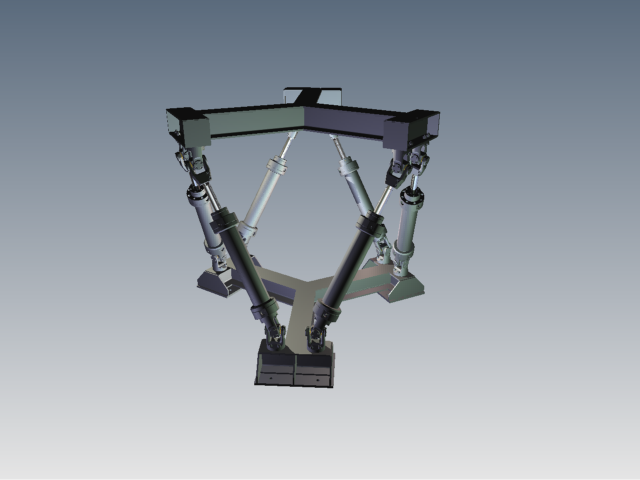
\includegraphics[scale=0.5]{ch-2/image8}
	}
	\caption{Пример платформы Стюарта.}\label{fig:stuart}
\end{figure}

Исполнительное устройство или рабочий орган размещаются на верхней плите и в определенном диапазоне линейных и угловых перемещений имеют шесть степеней свободы: линейное перемещение по осям x, y и z, а также вращения вокруг этих осей (крен, тангаж и рысканье).

К основным достоинствам данной кинематической схемы можно отнести:
\begin{itemize}
	\item Уже упомянутые ранее \textit{шесть степеней свободы}. Подобная конструкция позволяет рабочему органу двигаться по любой трехмерной траектории, что, безусловно, очень важно при создании таких типов оборудования как фрезерные металлорежущие станки и контрольно-измерительные машины.
	
	\item \textit{Высокая точность перемещения и повторяемость}. В отличие от других систем позиционирования любое перемещение платформы Стюарта требует изменения положения всех линейных приводов, что позволяет автоматически компенсировать механические погрешности, так как люфт не накапливает в какой-то одной координате, и может быть программно скомпенсирован на следующем этапе перемещения.
	
	\item \textit{Высокая жесткость конструкции}. Платформа Стюарта обеспечивает очень высокую жесткость своих механических компонентов и всех движущихся частей: подшипников, сочленений и приводных винтов (если они есть). Эта особенность позволяет достичь очень высоких значений собственной частоты конструкции (порядка~\SI{500}{\hertz} на~\SI{10}{\kilogram} нагрузки). Последнее означает, что построенные на базе платформы Стюарта металлорежущие станки могут работать на очень высоких скоростях резания. Кроме того, высокая жесткость конструкции дает возможность предотвратить изгиб линейных приводов, обеспечивающих движение платформы.
	
	\item \textit{Большая масса рабочего органа}. Вес рабочего органа, размещенного на верхней плите платформы Стюарта, равномерно распределен на шесть параллельных стоек. Это означает, что каждая из них несет на себе всего лишь одну шестую общего веса. Кроме того, каждая стойка работает только на растяжение и сжатие, не испытывая при этом никаких радиальных нагрузок. Следовательно, нет необходимости делать эти стойки массивными (как это делается в других подобных конструкциях).
	
	\item \textit{Большое разнообразие размеров платформы}. Конструктивные особенности платформы позволяют создавать на ее базе машине самых разных размеров в зависимости от целей и~задач, поставленных перед ними. По сравнению с другими подобными много осевыми конструкциями количество деталей, необходимых для создания платформы Стюарта на треть меньше, что делает конструкцию легче и подвижнее.
	
	
\end{itemize}
Несмотря на все вышеописанные достоинства, платформа Стюарта не лишена недостатков. Перечислим наиболее значимые из них:
\begin{itemize}
	\item \textit{Высокое трение}. Трение в многочисленных шарнирах "--- основной недостаток платформы Стюарта. Коэффициент трения конструкции равен примерно~0,8. Этого достаточно для небольшого осевого изгиба стоек (из-за незначительного заклинивания механизма), который, безусловно, влияет на точность и повторяемость конструкции. Использование керамического покрытия шарниров и специальной смазки позволяет снизить коэффициент трения до 0,2, но это существенно удорожает конструкцию.
	
	\item Даже с обычными шарнирами \textit{платформа Стюарта является очень дорогой конструкцией}. Большая стоимость определяется необходимостью использования шести линейных приводов. Также требуется гораздо более сложная система управления, причем как в программном (для быстрого и точного перемещения рабочего органа требуется постоянный пересчет его координат и перевод их в систему координат платформы), так и в аппаратном (все эти расчеты необходимо производить в режиме реального времени, что влечет за собой необходимость использования специализированных цифровых процессоров сигналов и более производительных микроконтроллеров). 
	
	\item \textit{Длина стоек.} Длина опорных стоек напрямую влияет на точность исполнительного механизма. При увеличении длины точность резко уменьшается из-за возможности изгиба. Также, возвращаясь к предыдущему пункту, можно сказать, что чем длиннее стойки, тем более дорогими будут линейные приводы, обеспечивающие их перемещение, но увеличение рабочей области без увеличения длины стоек невозможно.
	
	\item \textit{Динамическое тепловое расширение}. Вне зависимости от типа на высоких скоростях неизбежно возникает нагревание линейных приводов стоек платформы. В процессе работы механизма все стойки работают синхронно, однако степень нагрузки каждой из них различается. Это ведет к неконтролируемому изменению длины стоек, что увеличивает случайную погрешность позиционирования и снижает его точность. Единственный способ борьбы с динамическим тепловым расширением "--- постоянный их мониторинг и прогнозирование теплового расширения каждой стойки в реальном времени с помощью конечноэлементного анализа с последующим вводом компенсирующих перемещений. Безусловно, это еще больше усложняет и удорожает конструкцию.
	
	\item \textit{Необходимость калибровки механизма}. Точность параллельного механизма зависит от множества характеристик, для платформы Стюарта существует порядка 100 различных параметров, которые должны быть учтены в процессе настройки и калибрования механизма прежде, чем он сможет точно позиционировать свой рабочий орган.
\end{itemize}

\begin{figure}[ht]
	\centerfloat{
		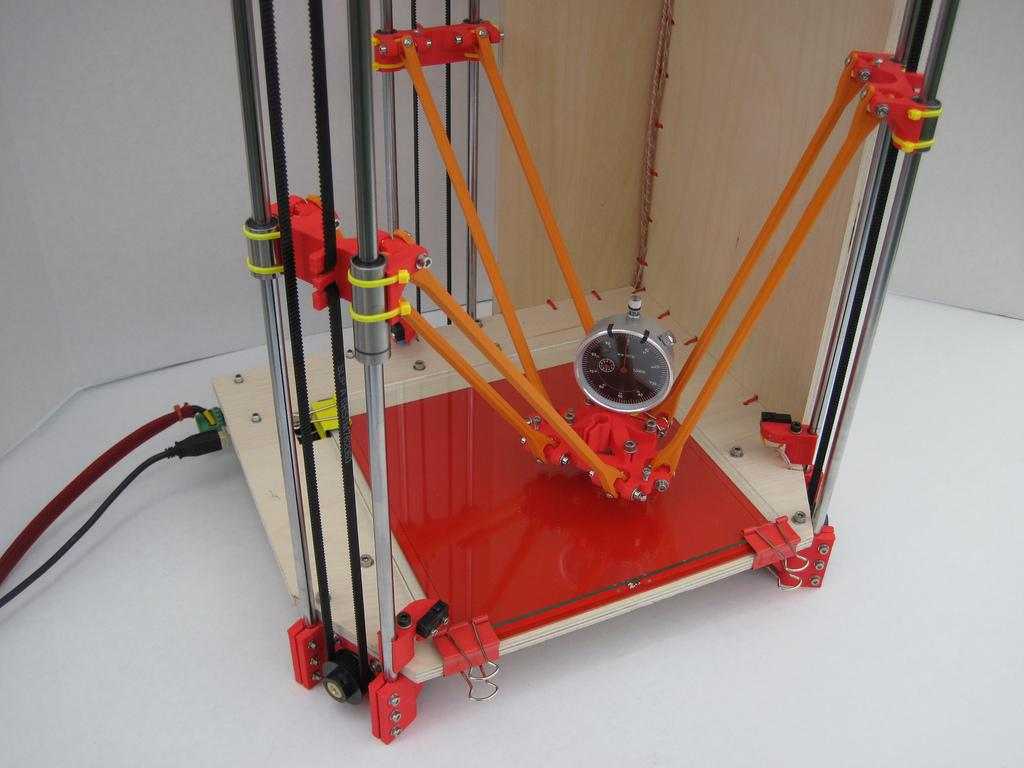
\includegraphics[scale=0.5]{ch-2/image9}
	}
	\caption{Дельта-робот.}\label{fig:delta}
\end{figure}

Помимо самой платформы Стюарта была также рассмотрена одна из ее разновидностей, а именно "--- дельта-робот~(рисунок~\cref{fig:delta}). Ключевой особенностью дельта-роботов является использование параллелограммов, положение которых задает перемещение рабочего органа дельта-робота.

В отличие от платформы Стюарта дельта-робот может позиционировать свой рабочий орган исключительно по трем основным координатам без вращений. Последнее существенно упрощает систему управления. Линейные приводы дельта-робота размещаются в~вертикальных стойках, что является его достоинством по сравнению с платформой Стюарта, так как линейные приводы не изменяют своей длины в процессе работы и подвержены минимальным осевым нагрузкам, что предотвращает их изгиб и позволяет увеличить жесткость конструкции.

Необходимо отметить, что рычажный механизм, связывающий каретки линейных приводов с креплением рабочего органа подвержен таким же нагрузкам, что и опоры платформы Стюарта, поэтому не исключен их изгиб под действием больших нагрузок. Единственный способ борьбы с этим явлением "--- увеличение массы стоек, что потребует существенного увеличения мощности линейных приводов и усложнения всей конструкции в целом. Также нельзя забывать, что рычаги соединяются с линейными приводами и креплением рабочего органа посредством цилиндрических шарниров (так как дельта-робот является разновидностью пантографа), надежность которых в жестких условиях эксплуатации является весьма сомнительной.

Как правило, рычаги делаются максимально легкими и жесткими за счет использования композиционных материалов, а сама конструкция чаще все находит применение в автоматических линиях, где требуется не высокая точность позиционирования, а большая скорость перемещения рабочего органа, которая для дельта-робота может достигать 10 м/с при ускорении до 30 g.

Получается, что ни одна из рассмотренных разновидностей механизма с параллельной кинематикой не удовлетворяем всем требованиям, предъявляемым к УШ, поэтому перейдем к рассмотрению следующего класса механизмов пространственного перемещения "--- координатным столам.

Координатный стол представляет собой мехатронную систему, сочетающую в себе несущую конструкцию и механизм многоосевоей подачи, обеспеченной наличием нескольких пространственно расположенных линейных приводов. Как правило, координатные столы работают в декартовой системе координат, что в отличие от описанных ранее механизмов с параллельной кинематикой не требует постоянного пересчета координат перемещения рабочего органа.

В качестве несущей конструкции координатных столов может быть использована станина или рама, выполненные в виде сварного или литого каркаса из конструкционной стали (обычно используются качественные углеродистые стали, например, Сталь20 или Сталь40), также станина может быть отлита из чугуна (в большинстве случаев это серый чугун марок СЧ~15-32 и СЧ~18-36) или выполнена из полимерного бетона. Литая конструкция является более предпочтительной, однако используется только в случае, когда координатный стол будет эксплуатироваться в особо жестких условиях, например в высокоскоростных металлорежущих станках, в остальных случаях чаще применяется сварная рама из стали.

Основное назначение станины "--- обеспечение жесткости конструкции стола и гашение вибрации, что напрямую связано с точностью и повторяемостью оборудования, использующего данный механизм пространственного перемещение.

Несущая конструкция связана с опорной рамой, выполненной из алюминиевого или стального проката. Функция опорной рамы "--- размещение на ней приводов и основной рабочей поверхности координатного стола.

Можно выделить как минимум два вида трёхкоординатных шасси~\cite{yang2013generalized, yang2015position}: \textit{крестового} типа и \textit{портального} типа. Крестовая конструкция~(рисунок~\cref{fig:cross}) обеспечивает большую гибкость и универсальность оборудования, построенного на ее основе, так как позволяет работать с объектами со сложной пространственной геометрией, когда необходимо обеспечить доступ к обрабатываемому объекту в верхней полуплоскости без пересечения траектории рабочего органа с элементами конструкции стола. В дополнение к этому, крестовая компоновка позволяет работать с объектами гораздо больше своего размера. Благодаря этому подобная конструкция нашла широкое применение в многокоординатных металлорежущих станках с ЧПУ.

\begin{figure}[ht]
	\centerfloat{
		\hfill
		\subcaptionbox{\label{fig:cross-1}}{%
			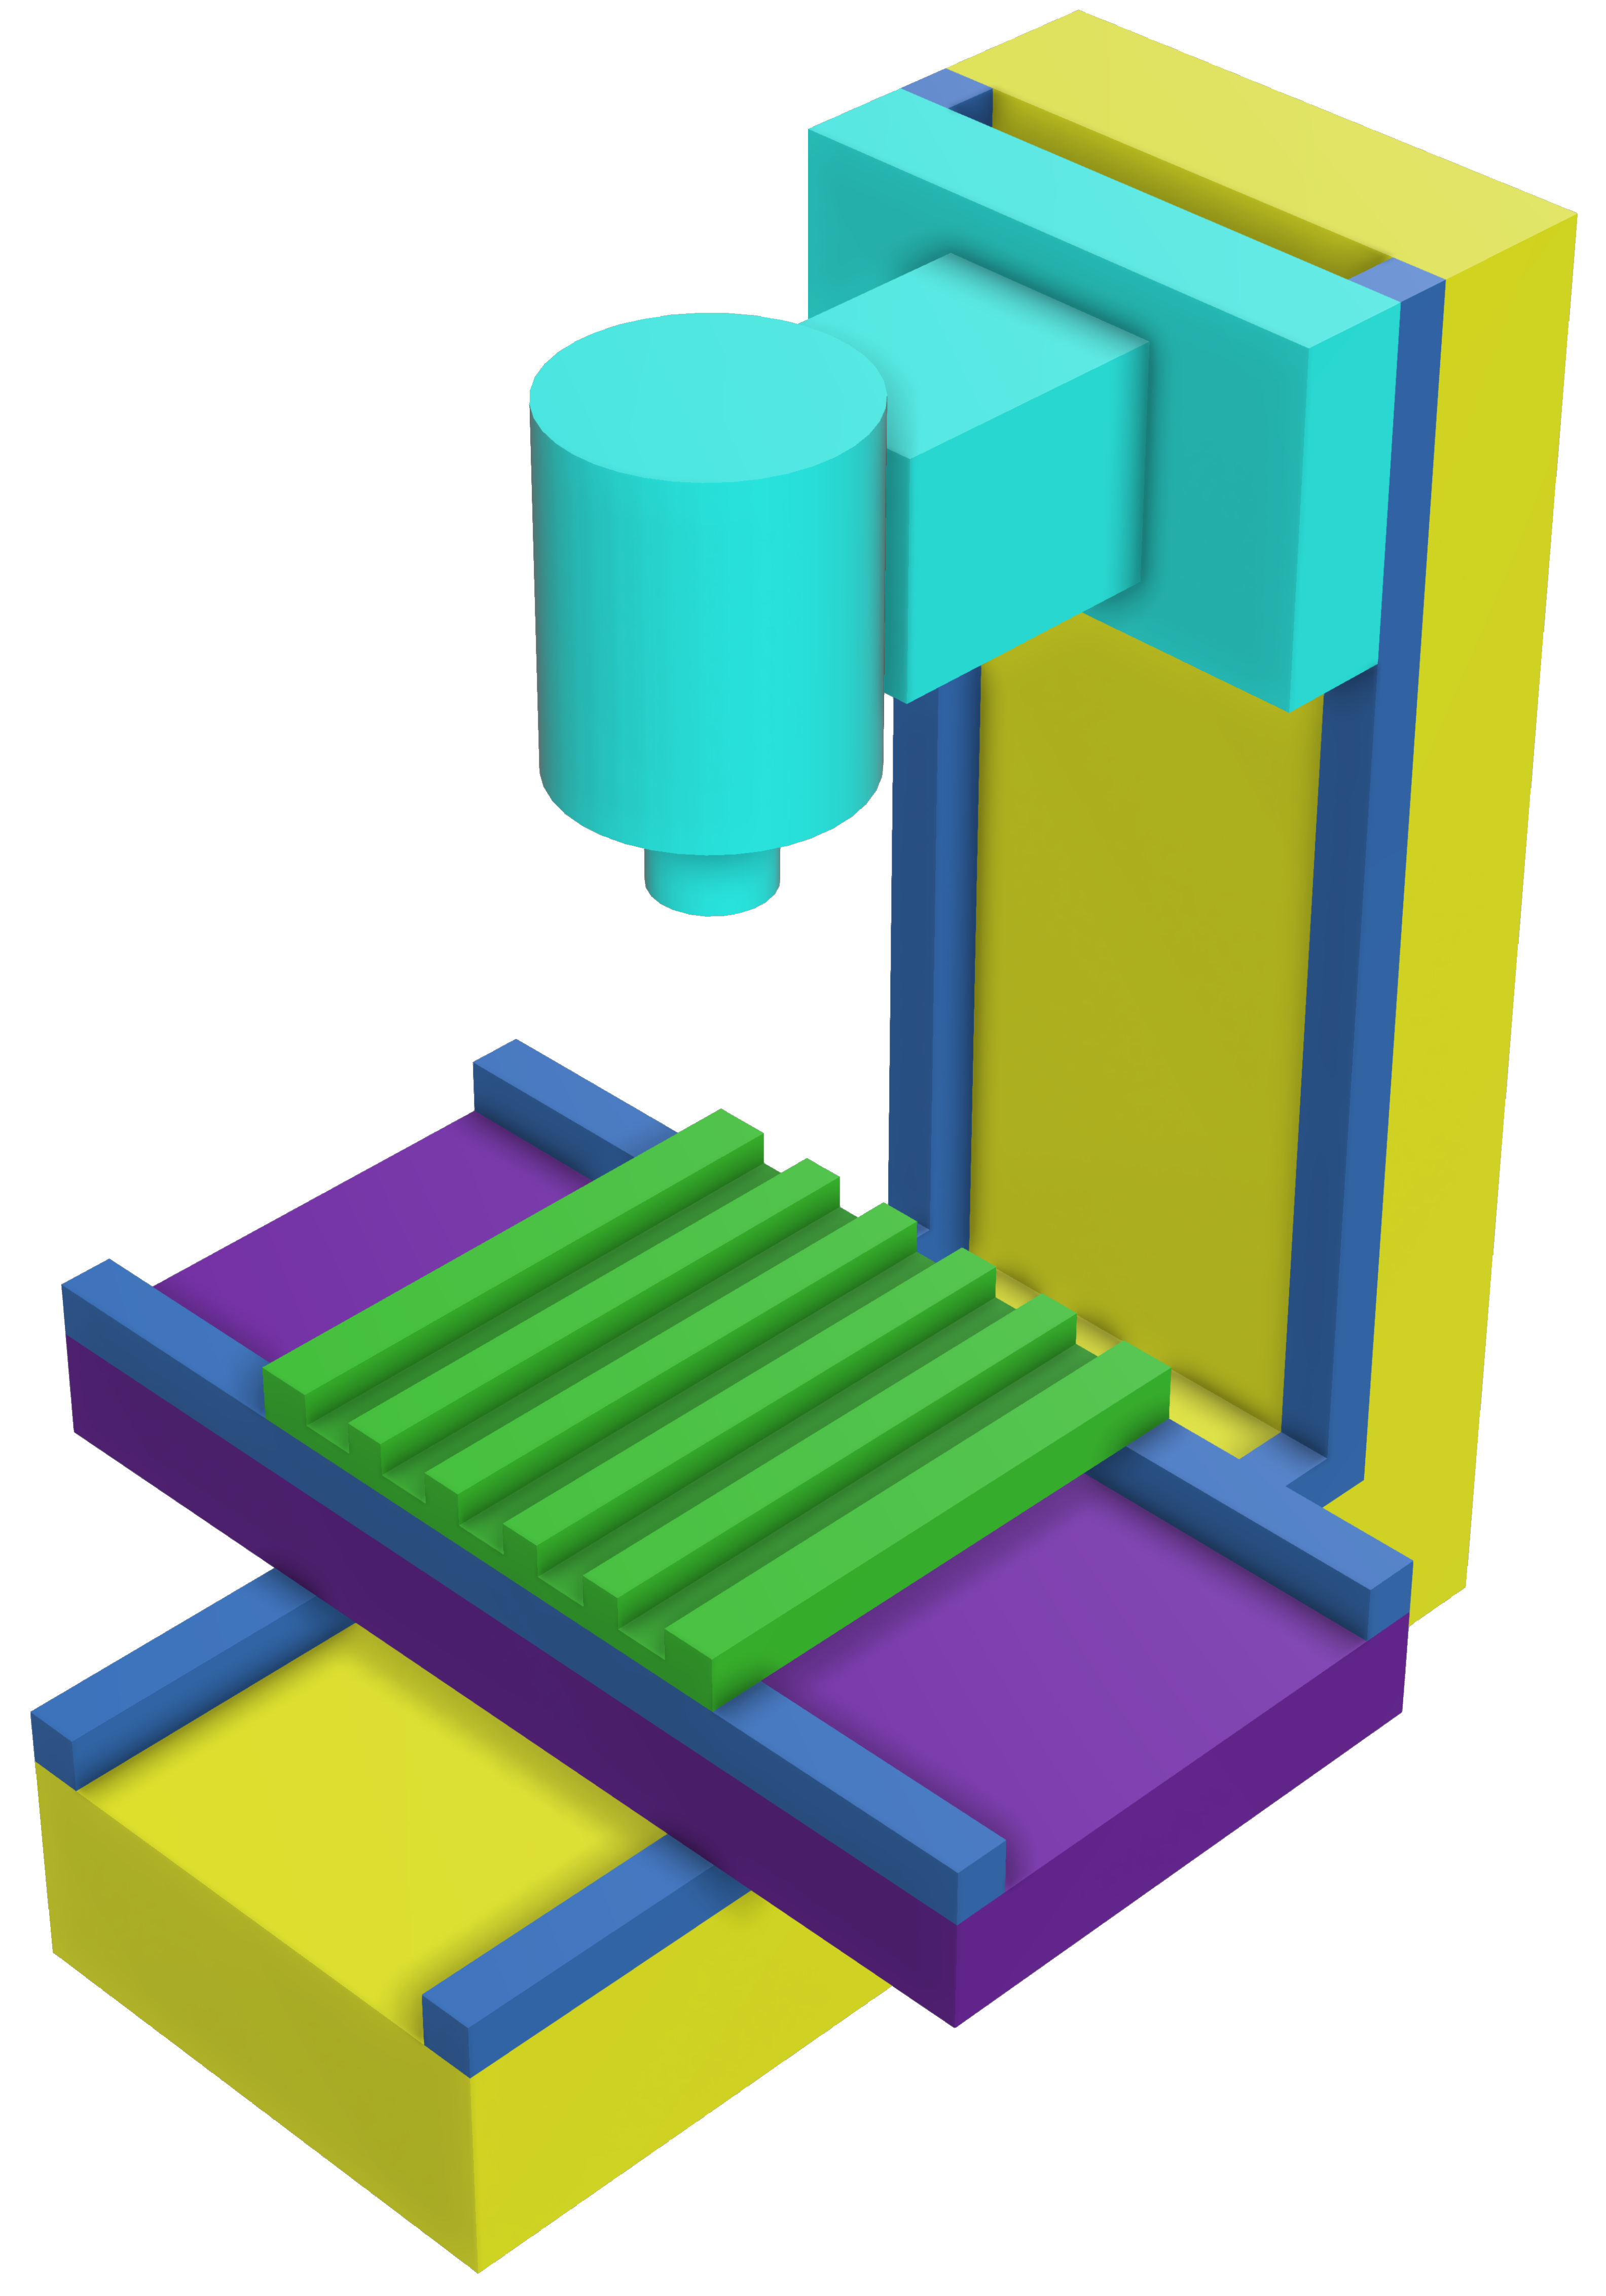
\includegraphics[width=0.33\linewidth]{ch-4/cnc-kin-4}}
		\hfill
		\subcaptionbox{\label{fig:cross-2}}{%
			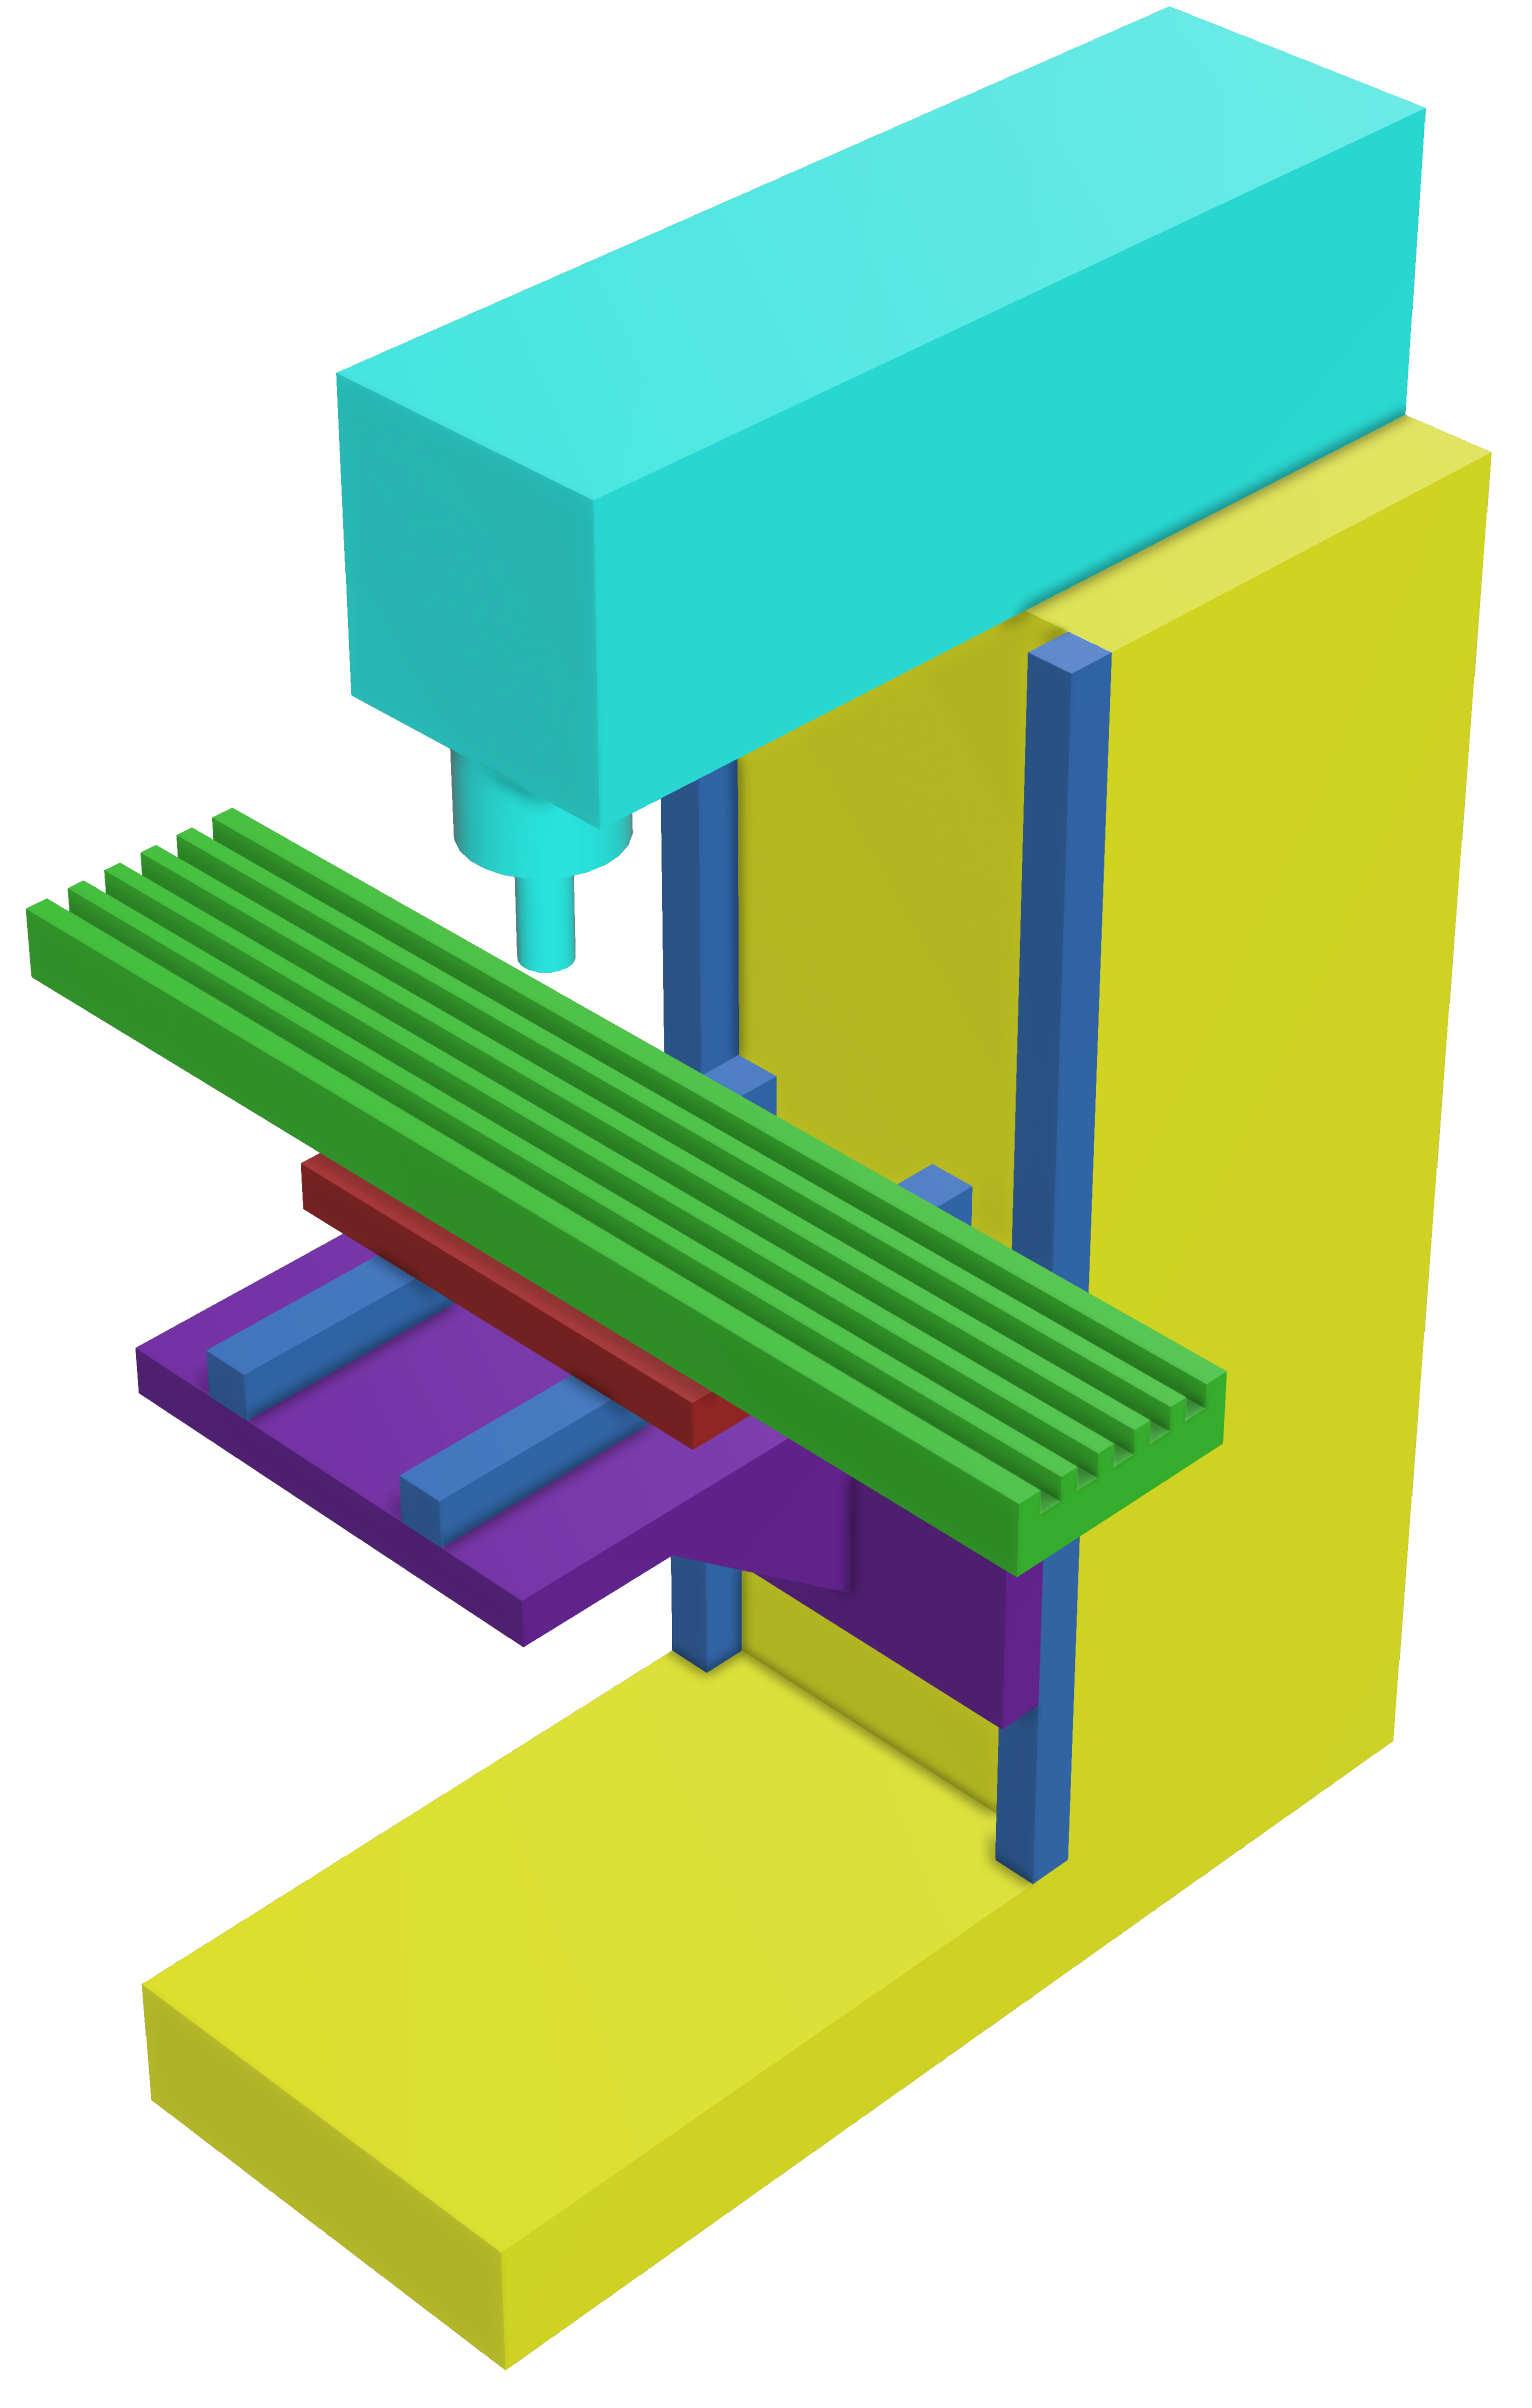
\includegraphics[width=0.33\linewidth]{ch-4/cnc-kin-6}}
		\hfill
		\subcaptionbox{\label{fig:cross-3}}{%
			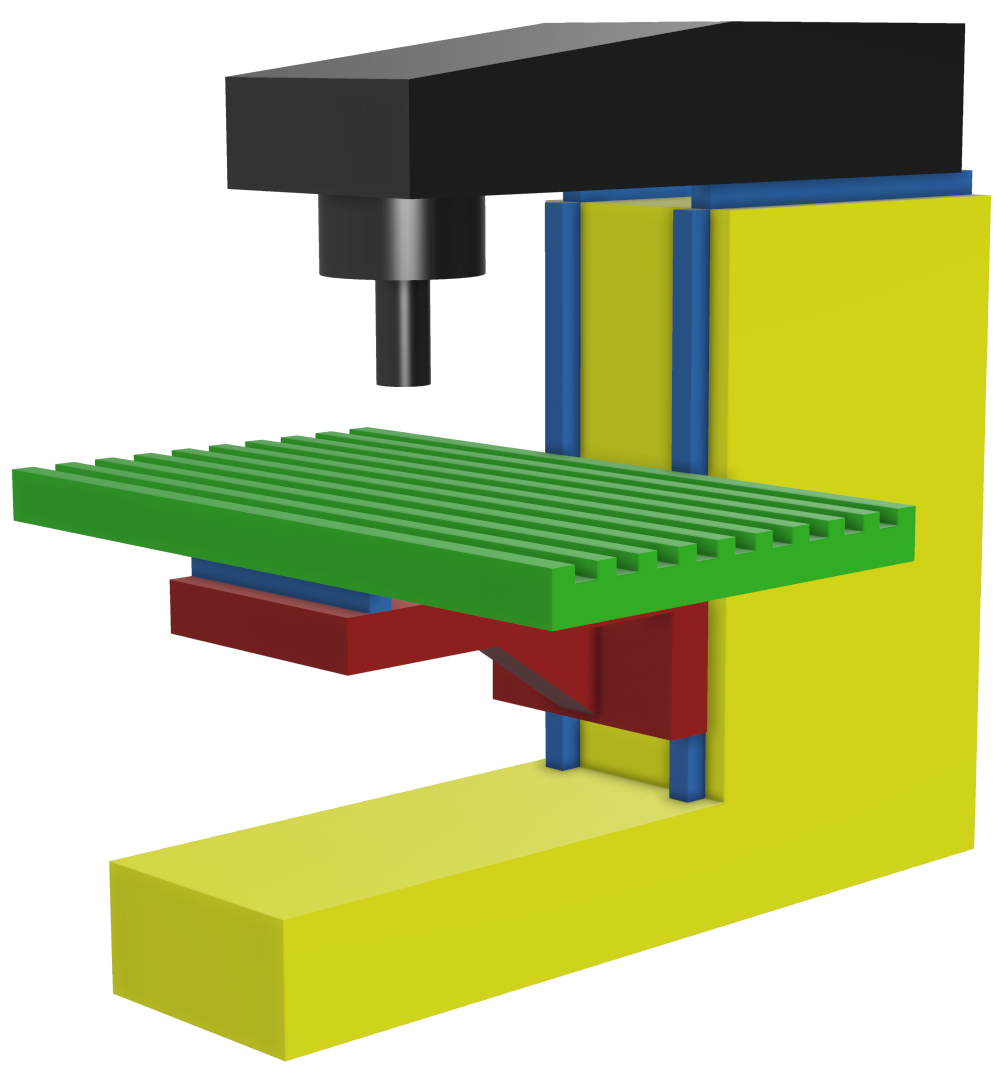
\includegraphics[width=0.33\linewidth]{ch-4/cnc-kin-7}}
		\hfill
	}
	\caption[Примеры конструкций трёхкоординатных шасси крестового типа с подвижным порталом]%
	{Примеры конструкций трёхкоординатных шасси крестового типа: бесконсольное исполнение с подвижной осью Z (\textit{а}), консольное исполнение с неподвижной осью Z  (\textit{б}), консольное исполнение с подвижной осью Y (\textit{в}).}\label{fig:cross}
\end{figure}

Можно выделить следующие недостатки крестовой конструкции координатных столов:

\begin{itemize}
	\item Данная кинематическая схема достаточно сложна в реализации, так как требует наличия жесткой связки линейных приводов, образующих рабочую крестовину.
	\item Увеличение массы перемещаемого объекта неизбежно ведет к необходимости увеличения мощности линейных приводов стола, что еще больше усложняет и удорожает конструкцию. Особенно это касается механизмов, где в дополнение к перемещению по координатам Х и Y, необходимо перемещение и по оси Z, то есть подъем или опускание крестовины относительно неподвижного рабочего органа. 
	\item Возможен прогиб осей по краям координатного стола.
\end{itemize}

Вторая разновидность координатных столов "--- портальная. Существует несколько компоновок портальных конструкций, отличающихся назначением и ограничениями областей применения. На рисунке~\cref{fig:fixed-portal-1} представлен координатный стол с неподвижным порталом, в~котором перемещение по оси Y осуществляется за счёт продольного движения самого стола, а рабочий орган расположен на траверсе, которая может опускаться и подниматься, обеспечивая тем самым, движение по оси Z. Перемещение по оси X достигается за счет наличия дополнительного линейного привода, также расположенного на данной траверсе.

К достоинствам данной конструкции можно отнести:

\begin{itemize}
	\item высокую жесткость на изгиб;
	\item простоту изготовления.
\end{itemize}

Недостатками являются:

\begin{itemize}
	\item отсутствие возможности работы с объектами большой массы, так как подобные объекты должны крепиться и перемещаться по оси Y, нагружая ее, что может привести к выходу из строя линейного привода или его изгиба.
	\item максимальные габаритные размеры объекта ограничены размером подвижного стола.	
\end{itemize}

Также существуют конструкции, где неподвижный портал несет на себе траверсу, отвечающую только за перемещение рабочего органа по координате Z~(рисунок~\cref{fig:fixed-portal-2}).

Перемещение по координатам X и Y, как видно из рисунка, осуществляется за счёт использования конструкции, похожей на крестовую, за исключением отсутствия единой точки крепления линейных приводов, что с одной стороны увеличивает жесткость конструкции и уменьшает прогиб по осям, а с другой "--- существенно сокращает рабочее поле стола.

Последний вариант конструкции с неподвижным порталом изображен на рисунке~\cref{fig:fixed-portal-3}. В данном механизме рабочий орган, размещенный на траверсе портала, обеспечивает перемещение по оси Y, в то время как рабочая поверхность может подниматься и опускаться (перемещение по оси Z), а также двигаться в поперечном по отношению к плоскости портала направлении (ось X). Очевидно, что подобная компоновка наиболее проста в реализации, но не является достаточно жесткой и не позволяет работать с объектами большой массы. Последнее определяет основную область применения данной кинематической схемы "--- изготовление недорогих трехмерных принтеров.

\begin{figure}[ht]
	\centerfloat{
		\hfill
		\subcaptionbox{\label{fig:fixed-portal-1}}{%
			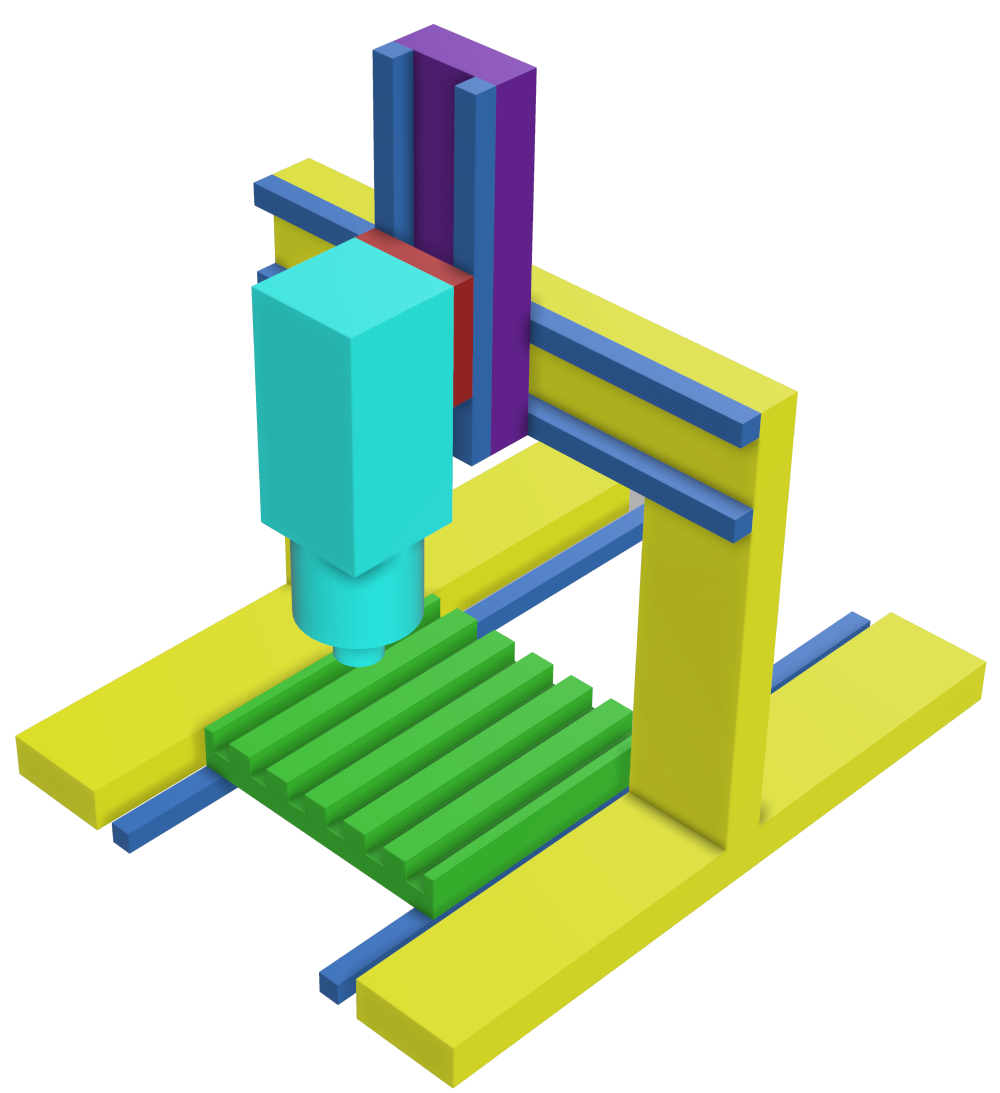
\includegraphics[width=0.33\linewidth]{ch-4/cnc-kin-3}}
		\hfill
		\subcaptionbox{\label{fig:fixed-portal-2}}{%
			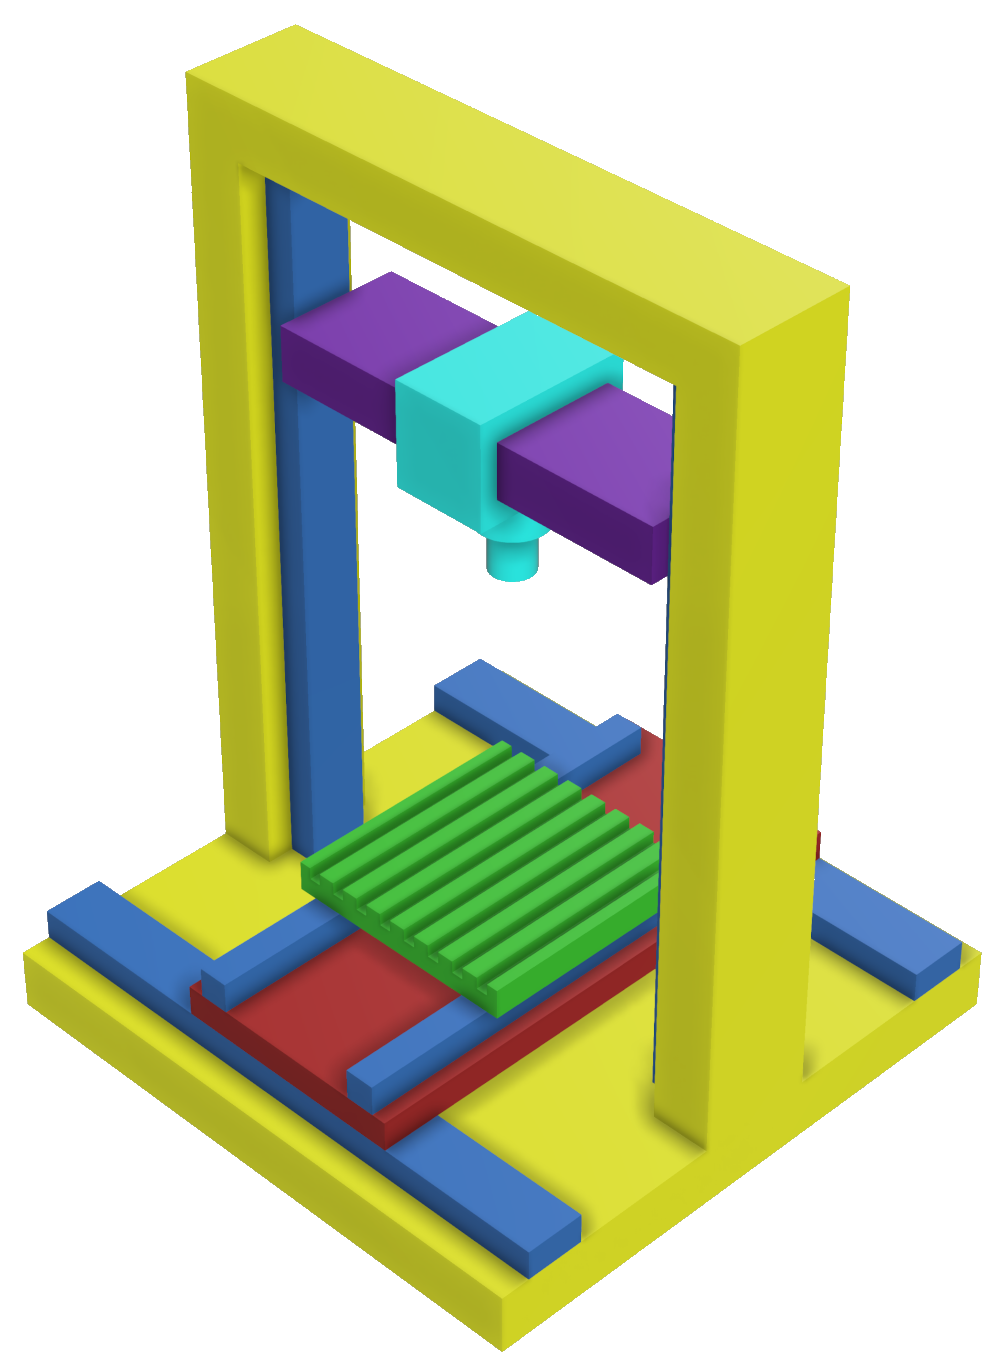
\includegraphics[width=0.33\linewidth]{ch-4/cnc-kin-9}}
		\hfill
		\subcaptionbox{\label{fig:fixed-portal-3}}{%
			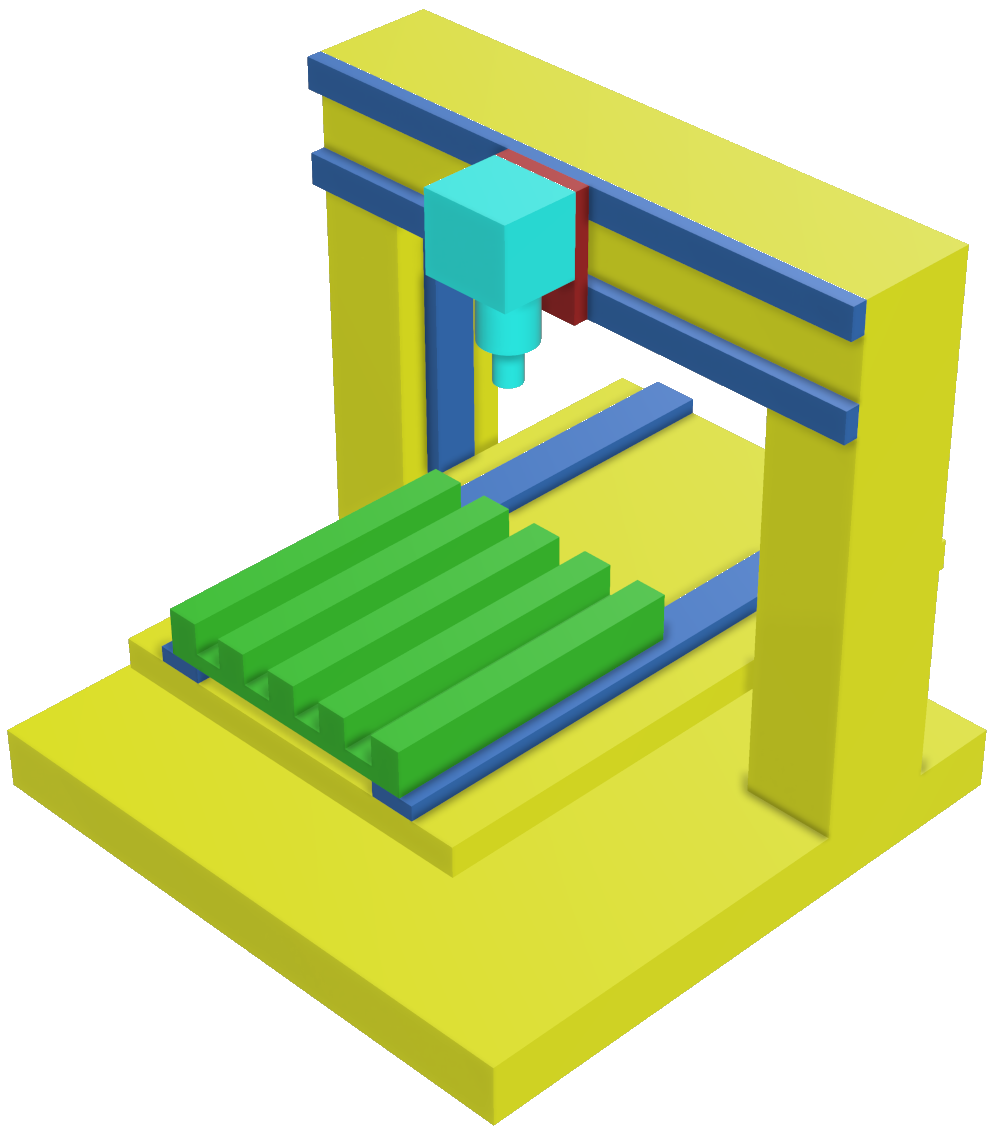
\includegraphics[width=0.33\linewidth]{ch-4/cnc-kin-8}}
		\hfill
	}
	\caption[Примеры конструкций трёхкоординатных шасси портального типа с неподвижным порталом]%
	{Примеры конструкций трёхкоординатных шасси портального типа с неподвижным порталом: исполнение с подвижным столом, обеспечивающим движение по оси Y и неподвижной траверсой, для перемещение в плоскости XZ (\textit{а}), исполнение с подвижным столом, обеспечивающим движение в плоскости XY и подвижной траверсой для перемещения по оси Z  (\textit{б}), консольное исполнение с подвижным по осям X и Z столом и неподвижной траверсой для перемещения по оси Y (\textit{в}).}\label{fig:fixed-portal}
\end{figure}

Отдельно следует рассмотреть конструкцию координатного стола с подвижным порталом~(рисунок~\cref{fig:move-portal}).

\begin{figure}[ht]
	\centerfloat{
		\hfill
		\subcaptionbox{\label{fig:move-portal-1}}{%
			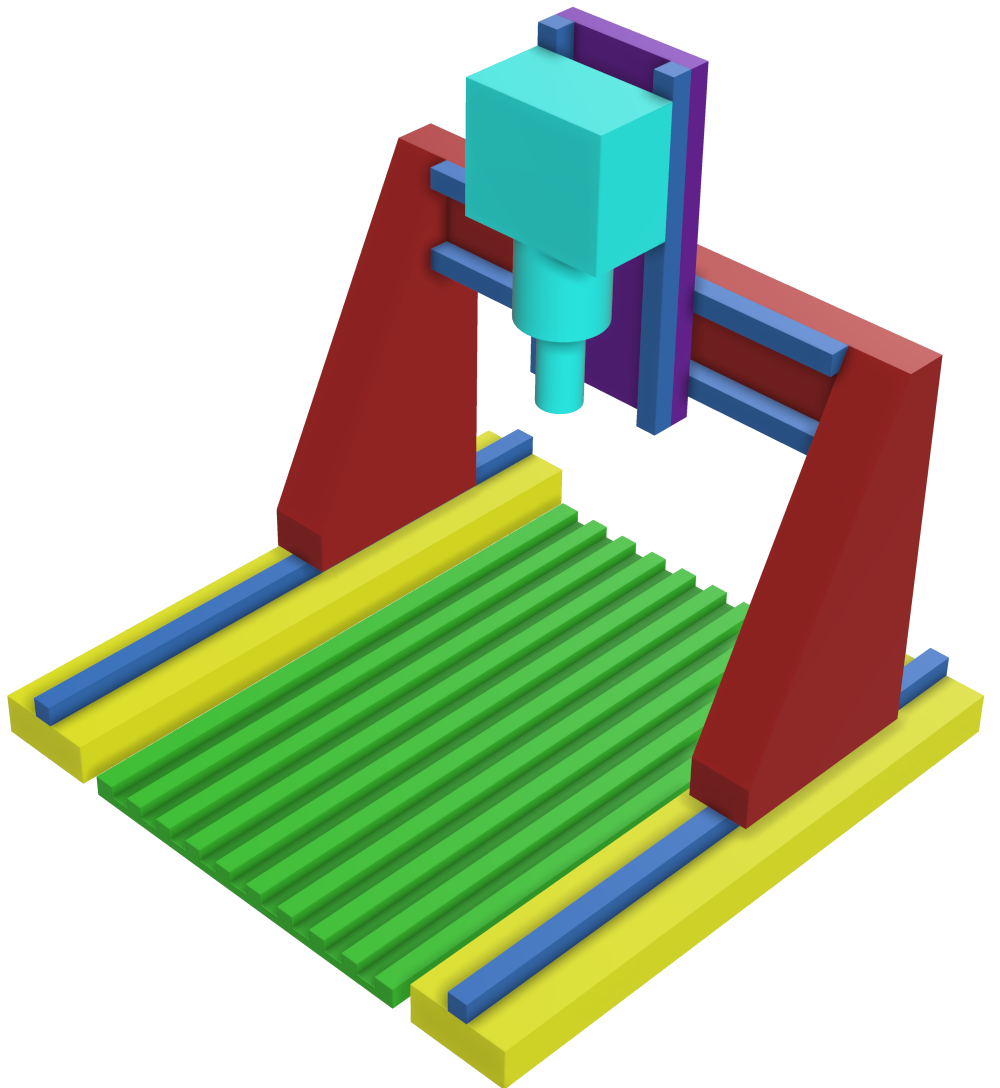
\includegraphics[width=0.33\linewidth]{ch-4/cnc-kin-5}}
		\hfill
		\subcaptionbox{\label{fig:move-portal-2}}{%
			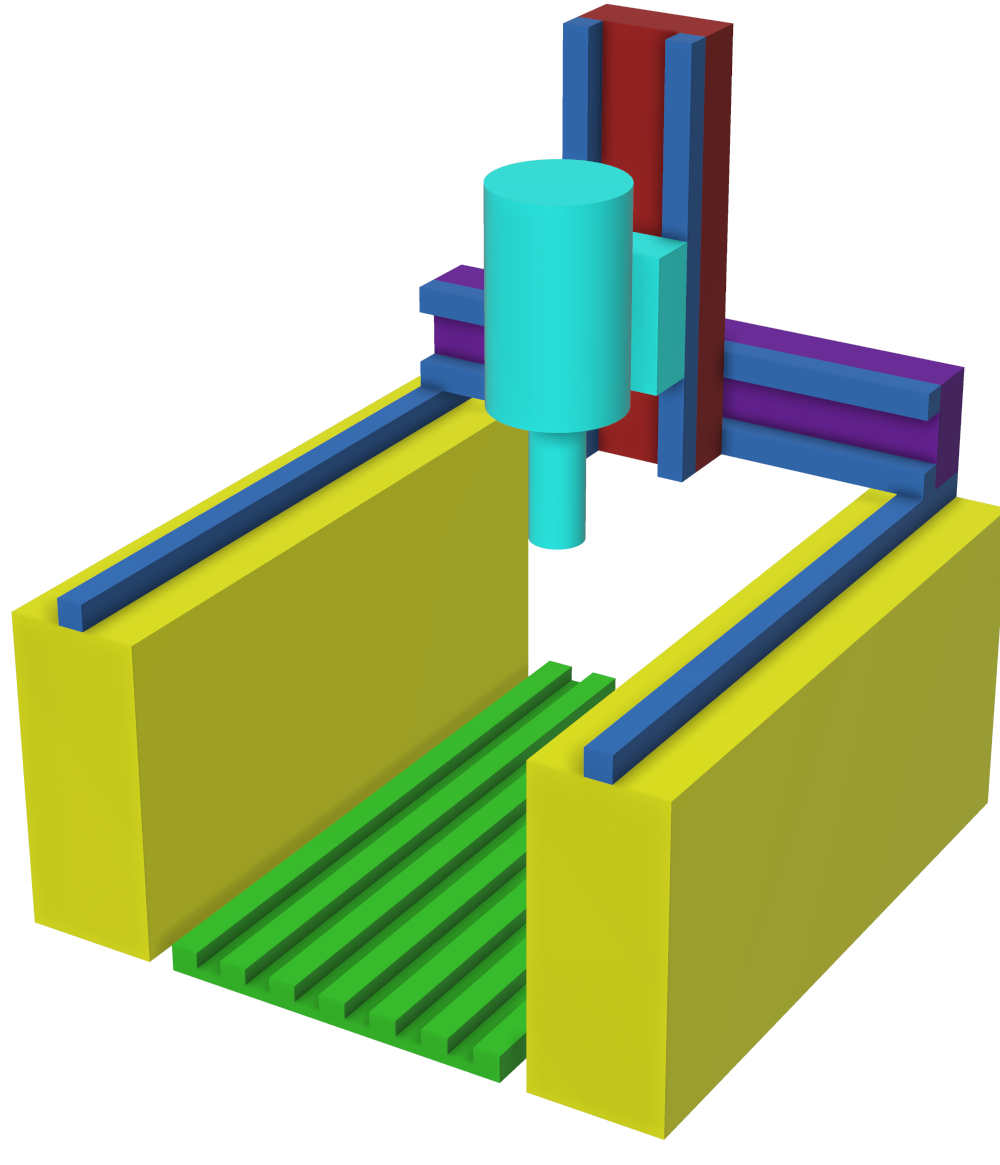
\includegraphics[width=0.33\linewidth]{ch-4/cnc-kin-1}}
		\hfill
		\subcaptionbox{\label{fig:move-portal-3}}{%
			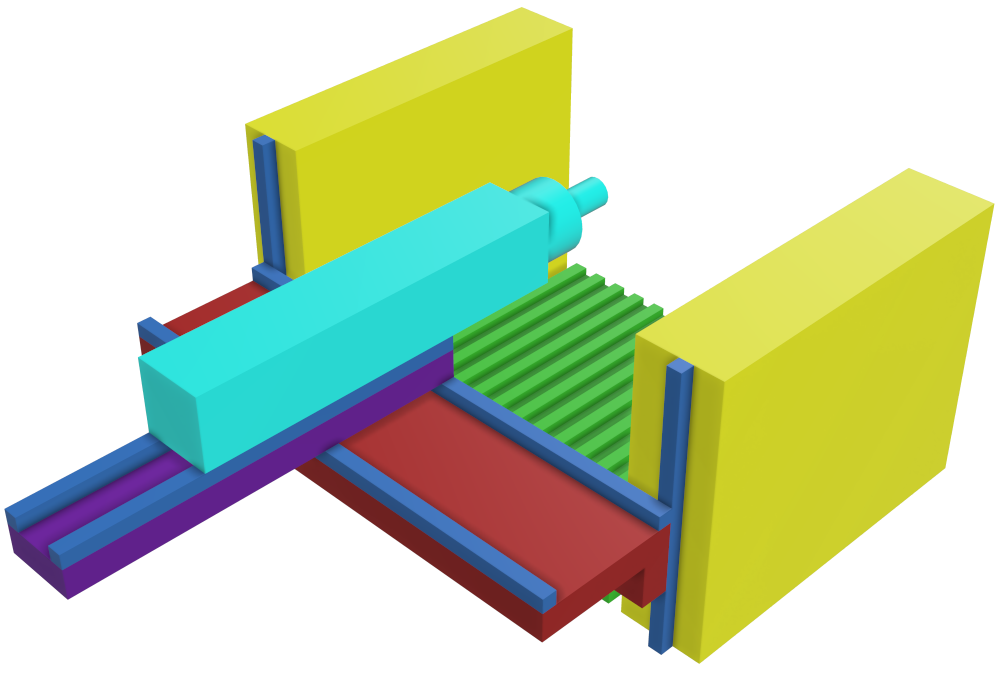
\includegraphics[width=0.33\linewidth]{ch-4/cnc-kin-2}}
		\hfill
	}
	\caption[Примеры конструкций трёхкоординатных шасси портального типа]%
	{Примеры конструкций трёхкоординатных шасси портального типа: исполнение с подвижным П-образным порталом (\textit{а}), исполнение с подвижной траверсой в плосткости XY  (\textit{б}), исполнение с подвижной траверсой в плоскости XZ (\textit{в}).}\label{fig:move-portal}
\end{figure}

Исполнение, представленное на рисунке~\cref{fig:move-portal-1} несколько сложнее предыдущих, так как сам портал и поперечная балка обеспечиваю перемещение рабочего органа по всем трем осям, рабочая поверхность стола при этом остается неподвижной. К очевидным достоинствам подобной кинематической схемы можно отнести:

\begin{itemize}
	\item достаточную простоту изготовления;
	\item универсальность и масштабируемость конструкции;
	\item ничем не ограниченный вес объекта;
	\item возможность встраивания в поточные линии (в качестве так называемого декартового робота);
	\item возможность работы с объектами, значительно превышающими габариты стола по оси Y, что находит применение при работе с листовыми материалами.
\end{itemize}

Основными недостатками конструкции являются:

\begin{itemize}
	\item необходимость использования очень жестких и прочных линейных приводов по оси Y, так как именно они будут испытывать максимальные нагрузки в процессе своей работы.
	\item зависимость жесткости и точности координатного стола от высоты портала, так как при увеличении размеров боковых стоек возможно увеличение их деформации и изгиба.
\end{itemize}

Анализ показал, что кинематическая схема координатного стола с подвижным порталом (рисунок~\cref{fig:move-portal-1}) является наиболее распространенной при создании металлообрабатывающих и деревообрабатывающих станков координатно-фрезерного и координатно-сверлильного типов, механических, водоструйных, лазерных и плазменных резаков, различных граверов и режущих плоттеров и многих других видов оборудования с числовым программным управлением. Конструкция с подвижным порталом (рисунок~\cref{fig:move-portal-3}) чаще всего используется в крупных обрабатывающих центрах, где требуется максимальный объем рабочего пространства внутри закрытой камеры станка. При этом данная конструкция достаточно сложна в реализации, так как в ней ось шпинделя должна быть размещена консольно с большим вылетом, что существенно увеличивает габаритный размер полученного станка в плане. При этом конструкция (рисунок~\cref{fig:move-portal-1}) является наиболее универсальной, так как по сути состоит из рамы, которая обеспечивает перемещение по осям X и Y. Данная рама с линейными приводами может быть изготовлена и собрана отдельно, а затем установлена на основание станка, при этом габарит рабочей зоны по оси Z может варьироваться за счёт установки неподвижного стола на разную высоту.

По совокупности достоинств и недостатков именно данная конструкция была принята в качестве наиболее близкого аналога кинематической схемы УШ. Однако для многих типов оборудования, разрабатываемых в соответствии с концепцией МТП, третья координата вообще не требуется, для некоторых требуется, но с малым ходом и точностью, и лишь для самых сложных видов оборудования необходима полноценная высокоточная третья координата. В связи с этим в кинематической схеме УШ должна быть предусмотрена возможность регулировки рабочего стола по высоте, что позволит достичь максимальной точности и жесткости конструкции, сохранив при этом достаточно большие габариты рабочей области, а опциональную третью координату выполнить в качестве отдельного агрегата, на котором будет крепиться рабочий орган~(рисунок~\cref{fig:coord-chassis}).

\begin{figure}[ht]
	\centerfloat{
		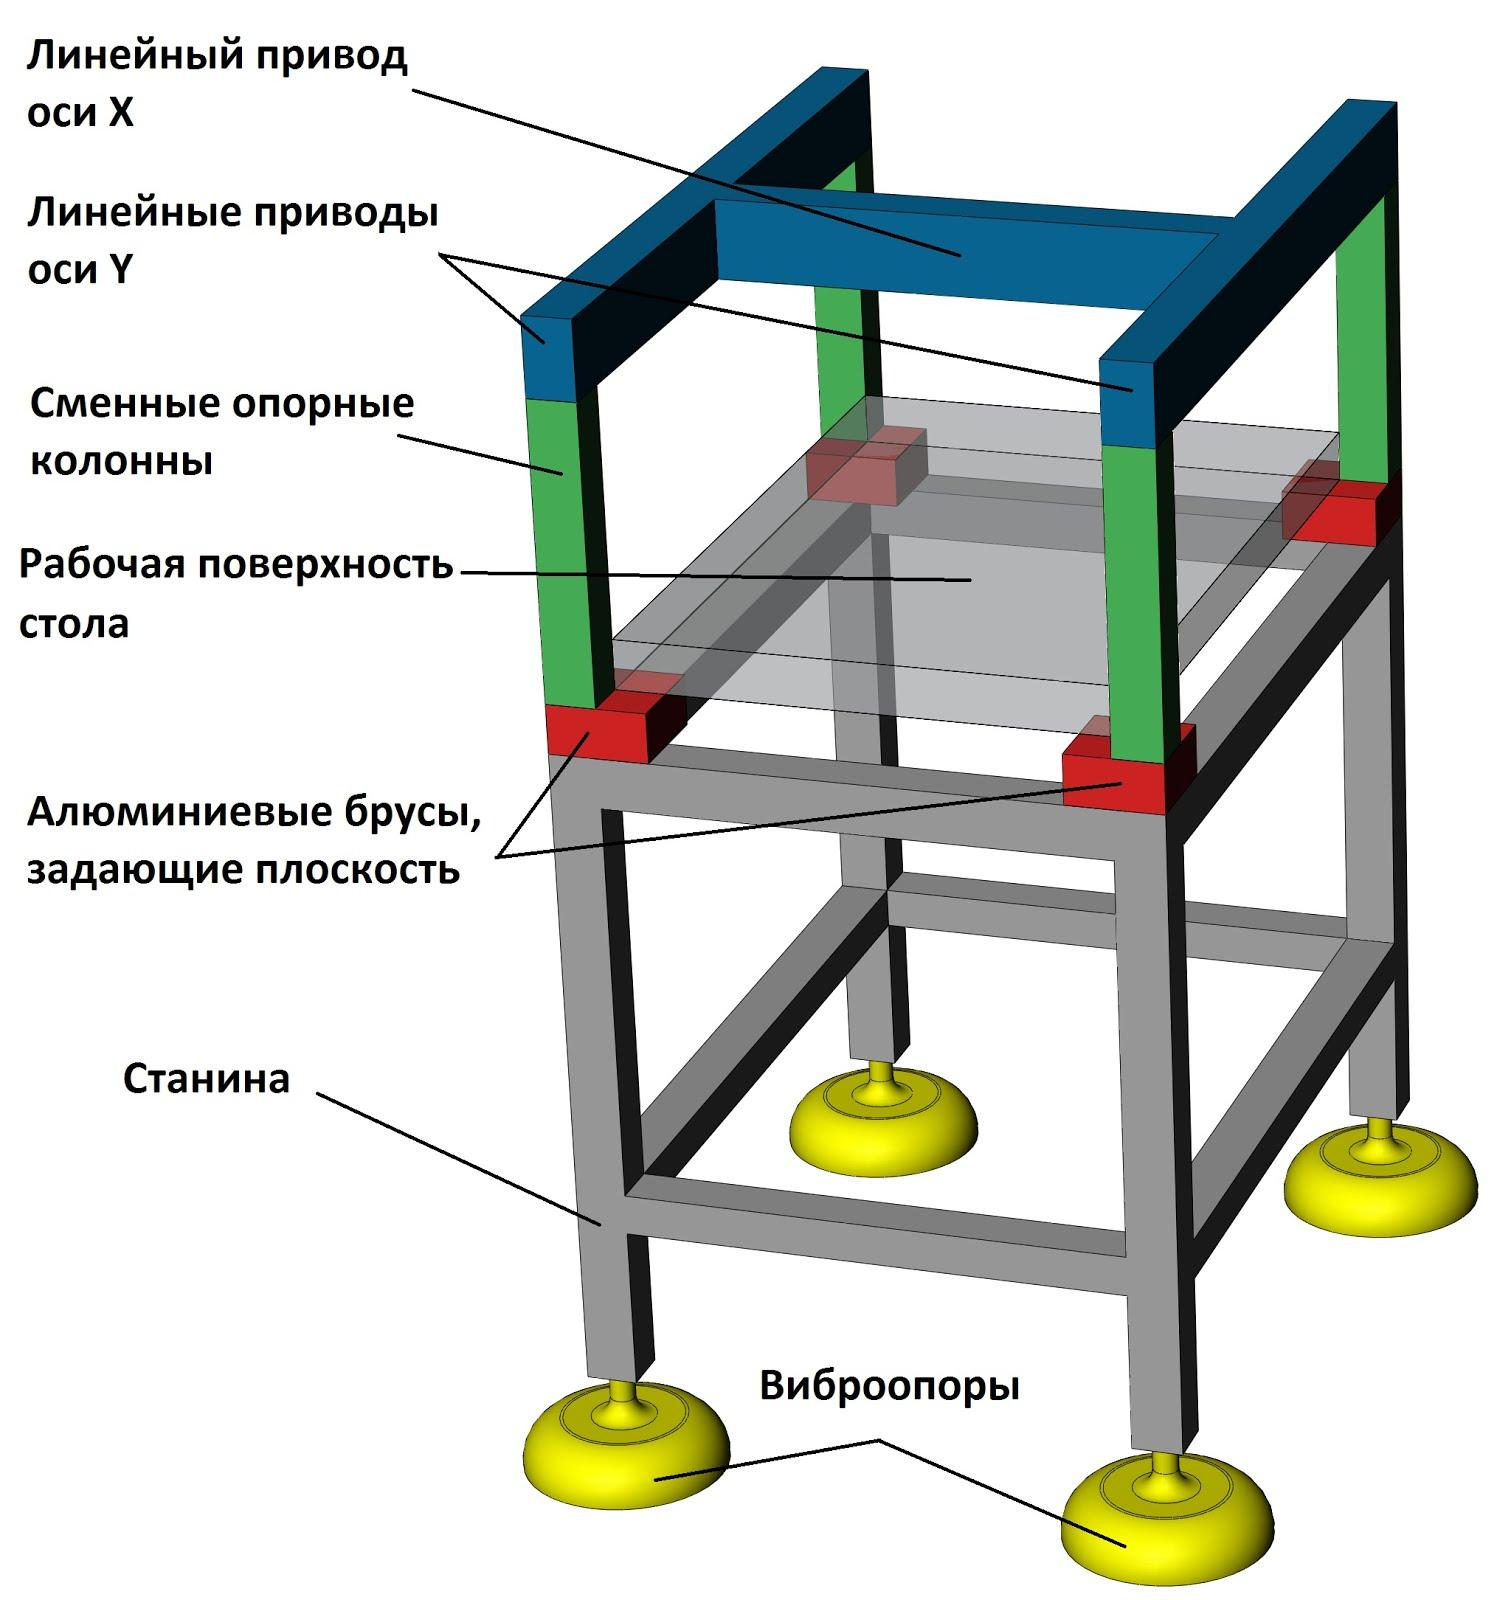
\includegraphics[width=0.7\textwidth]{ch-2/image15}
	}
	\caption{Общая компоновка УШ.}\label{fig:coord-chassis}
\end{figure}

Основание портала (станина) представляет собой сварную раму из стального проката (прямоугольные или квадратные трубы), по углам которой болтами необходимо закрепить четыре алюминиевых бруска, фрезеруемые совместно уже после крепления на раму. Бруски обеспечат плоскость, относительно которой можно базировать рабочую поверхность координатного стола и сменные опорные колонны, на которые будут опираться продольные и поперечные линейные приводы. Станина установлена на регулируемые по высоте виброопоры типов ОВ-31 и ОВ-70~(рисунок~\cref{fig:vibro}) в зависимости от общего веса конструкции.

\begin{figure}[ht]
	\centerfloat{
		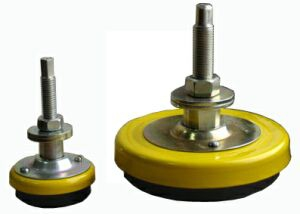
\includegraphics[width=0.7\textwidth]{ch-2/image16}
	}
	\caption[Виброопоры ОВ-31 и ОВ-70]{Виброопоры ОВ-31 (слева) и ОВ-70 (справа)}\label{fig:vibro}
\end{figure}

\subsection{Выбор линейных приводов универсального шасси}

Линейный привод представляет собой конструкцию, являющуюся совокупностью механизмов, предназначенных для линейного перемещения исполнительных органов машин и приборов. В зависимости от вида преобразуемой энергии различают следующие виды линейных приводов:

\begin{itemize}
	\item линейные электроприводы;
	\item линейные гидроприводы;
	\item линейные пневмоприводы.
\end{itemize}

С точки зрения управления и реализации самыми простыми являются электроприводы, поэтому для реализации перемещения рабочего органа УШ будут применяться именно они.

Линейный привод состоит из трансмиссии, преобразующей вращательное движение в поступательное, и электродвигателя. Отдельно можно выделить линейный электродвигатель (или просто линейный двигатель).

\textit{Линейный двигатель}~(рисунок~\cref{fig:lindrive}) "--- это электродвигатель, один из элементов магнитной системы которого линейно развернут (он создает магнитное поле), а другой выполнен в виде подвижной каретки, перемещающейся в этом поле. На сегодняшний день существует несколько разновидностей линейных двигателей: линейные асинхронные электродвигатели, линейные синхронные электродвигатели, линейные электромагнитные двигатели, линейные магнитоэлектрические двигатели, линейные магнитострикционные двигатели, линейные пьезоэлектрические (электрострикционные) двигатели и~др.

\begin{figure}[ht]
	\centerfloat{
		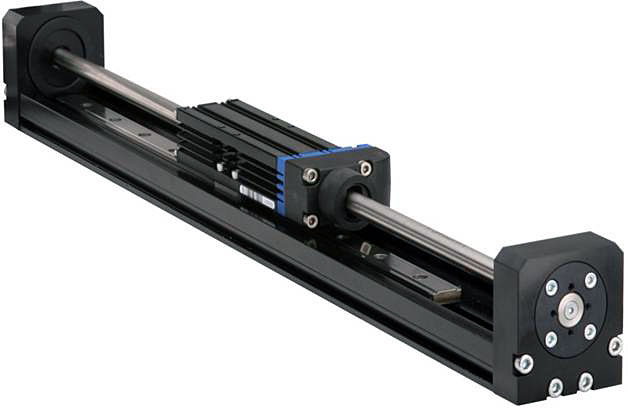
\includegraphics[width=0.7\textwidth]{ch-2/image17}
	}
	\caption{Цилиндрический линейный двигатель на постоянных магнитах.}\label{fig:lindrive}
\end{figure}

Основными достоинствами линейных двигателей являются:

\begin{itemize}
	\item \textit{Высокая скорость перемещения.} Максимальная скорость перемещения линейного двигателя ограничена только напряжением питания и производительностью управляющего контроллера (то есть его возможностью генерировать управляющие импульсы с максимально высокой частотой). Типичная скорость перемещения каретки линейного двигателя составляет 3 м/с при точности позиционирования 1 мкм и до 5 м/с при уменьшении точности. Очевидно, что для многих типов оборудования, проектируемого в рамках концепции МТП, подобная скорость движения исполнительного органа будет избыточной.
	
	\item \textit{Высокая точность.} Точность, разрешающая способность и~повторяемость "--- те характеристики линейного двигателя, которые определяются обязательной для данного вида линейных приводов системой обратной связи по положению. Как правило, используются различные линейные системы контроля положения, выбор которых зависит в первую очередь от назначения и стоимости устройства, построенного на базе линейного двигателя.
	
	\item \textit{Очень высокое ускорение} (время разгона до номинальной скорости). Быстродействие линейного двигателя примерно в~сто раз больше, чем у аналогичных линейных электроприводов с трансмиссией, что позволяет использовать его в наиболее требовательных к этому параметру системах.
	
	\item \textit{Высокая жесткость.} В линейных двигателях отсутствует трансмиссия, поэтому жесткость, как характеристика сопротивления каретки линейного двигателя внешнему воздействию, может быть увеличена только за счет увеличения тока в обмотках якоря. Правда это увеличение не может быть бесконечно и зависит от сопротивления изоляции обмоток, системы охлаждения, необходимой точности позиционирования и т.\:д.
	
	\item \textit{Отсутствие люфта.} В линейных двигателях отсутствует свободный ход каретки по отношению к направляющей, что определяется отсутствием механической трансмиссии. Все ошибки позиционирования возникают только из-за несовершенства блока управления, система обратной связи по положению и качества изготовления деталей, генерирующих магнитное поле. Эти ошибки носят систематический характер и могут быть учтены в программе управления. 
\end{itemize}

Несмотря на все перечисленные достоинства, линейные двигатели не лишены и определенных недостатков. Перечислим те из них, которые по нашему мнению не позволяют использовать данный тип линейных приводов при создании УШ:

\begin{itemize}
	\item \textit{Стоимость}. Линейные двигатели стоят очень дорого. В~первую очередь это связано с необходимостью использования дорогих редкоземельных магнитов. Лучшие и~самые дорогие модели линейных двигателей создаются на базе цилиндрических направляющих (рельсов) с постоянными магнитами, расположенными по всей длине рельса. Очевидно, что стоимость такого привода растет пропорционально длине магнитных направляющих. Второй немаловажный фактор, влияющий на цену линейных двигателей "--- обязательная необходимость использования линейных датчиков, обеспечивающих обратную связь по положению. Данный тип датчиков является наиболее сложным и дорогим. Также стоит отметить, что линейные двигатели, как правило, требуют более сложного блока управления, построенного не на основе микроконтроллеров общего назначения, а на более дорогих цифровых процессорах сигнала (англ. \textit{Digital Signal Processor}, сокр. \textit{DSP}).
	
	\item \textit{Низкое тяговое усилие.} В сравнении с идентичными по массогабаритным характеристикам вращающимися двигателями, линейные двигатели развивают значительно более низкое тяговое усилие.
	
	\item \textit{Высокая рабочая температура.} В большинстве линейных двигателей якорь напрямую соединен с нагрузкой. КПД линейного двигателя может достигать 96\%, 4\% уходит в тепло, которому необходимо где-то рассеяться, поэтому в линейных двигателях высокой мощности обязательными являются системы принудительного воздушного или водяного охлаждения.
	
	\item \textit{Практически полное отсутствие трения.} В рабочем режиме якорь линейного двигателя находится в состоянии магнитной левитации, трение при этом минимально (только трение о~воздух). С одной стороны это достоинство линейных двигателей, а с другой "--- отсутствие трения означает и~отсутствие самоторможения. Например, представим вертикально расположенный линейный двигатель, якорь которого соединен с некоторой полезной нагрузкой и в данный момент находится в режиме удержания. Что произойдет в~случае потери питания? Если сила тяжести, действующая на якорь с закрепленной на нем полезной нагрузкой, окажется выше силы удержания постоянных магнитов в отсутствие магнитного поля, создаваемого катушками якоря, он просто упадет. Другой пример, якорь с полезной нагрузкой движется с максимальной скоростью (5 м/с), опять же происходит потеря питания. Единственное, что может остановить якорь "--- сила трения скольжения, возникающая между внутренней поверхностью якоря и доведенной поверхностью рельса. Очевидно, что при незначительной длине рельса ее будет недостаточно для быстрой остановки якоря, он ударится о концевую планку и может быть разрушен вместе с полезной нагрузкой.
	
	\item \textit{Высокое энергопотребление}. Анализ характеристик линейных двигателей показал, что при одинаковом тяговом усилии линейные двигатели потребляют больше электроэнергии, чем их вращающиеся аналоги.
	
	\item \textit{Не подлежат замене и модернизации.} Линейный двигатель является составной частью механизма, в котором он используется. Очевидно, что его крайне сложно заменить или модернизировать. Последнее явно противоречит принципу модульности, которому должно соответствовать оборудование, создаваемое в соответствии с концепцией МТП.
\end{itemize}

Как уже было сказано ранее, \textit{линейные электроприводы с~трансмиссией} представляют собой совокупность механизма преобразующего вращательное движение двигателя в поступательное "--- цепи, зубчатого ремня, винтовой или шарико-винтовой пары (сокр. ШВП) и двигателя "--- шагового или серво. Рассмотрим эти элементы более подробно.

\textit{Цепная передача} осуществляет преобразование вращательно движения за счет использования специального многозвенного гибкого механизма, именуемого цепью. Связь цепи с валом электродвигателя осуществляется благодаря силам зацепления так называемой ведущей звездочки, также в конструкции должна быть предусмотрена вторая (ведомая звездочка), вращающаяся свободно и необходимая для создания замкнутого контура вращения и натяжения цепи. Количество зубьев в ведомой и ведущей звездочках должно совпадать, так как не требуется преобразование момента силы (передаточное отношение 1:1). При использовании цепной передачи каретка линейного привода перемещается по направляющим (рельсовым или цилиндрическим) и жестко связана с цепью. В случае большой нагрузки на линейный привод допускается использования многорядных цепей~(рисунок~\cref{fig:chain}).

\begin{figure}[ht]
	\centerfloat{
		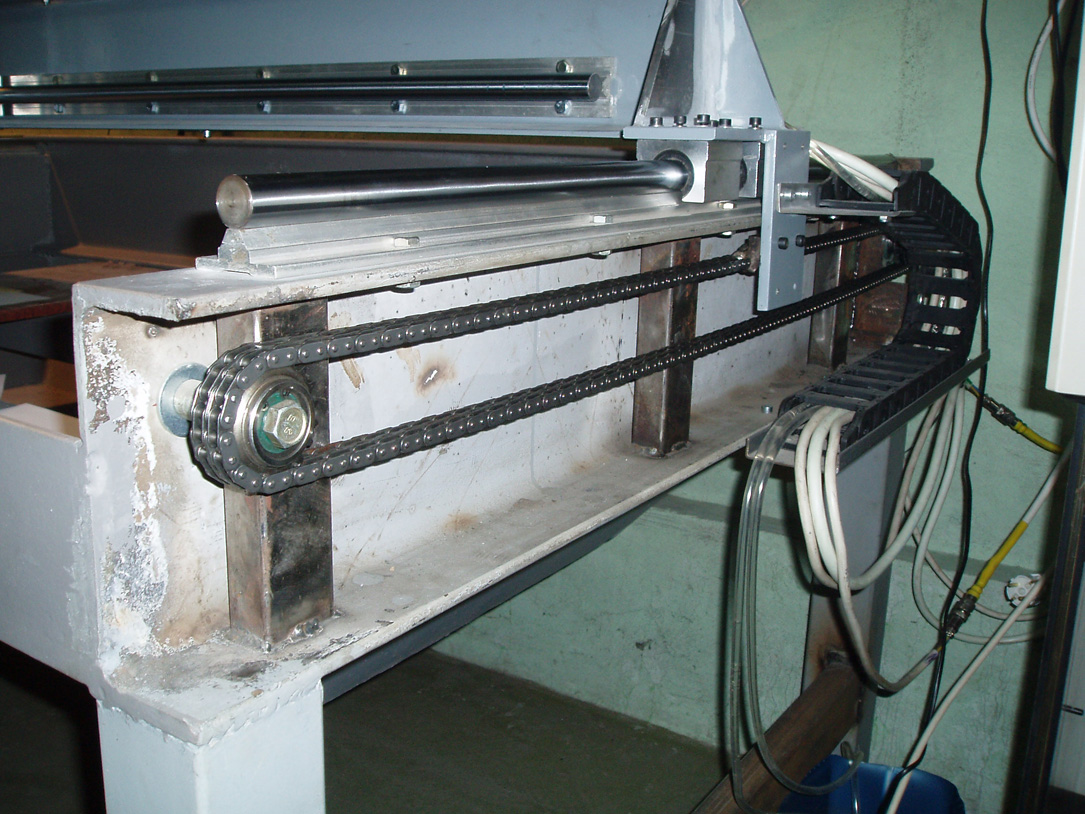
\includegraphics[width=0.7\textwidth]{ch-2/image18}
	}
	\caption{Пример многорядного цепного линейного привода.}\label{fig:chain}
\end{figure}

К достоинствам цепного линейного привода можно отнести:

\begin{itemize}
	\item Большая механическая прочность стальной цепи, позволяющая создавать высоконагруженные линейные приводы.
	
	\item Возможность создания достаточно габаритных линейных приводов.
	
	\item Достаточно высокий КПД (вплоть до 98\%).
	
	\item Отсутствие проскальзывания цепи.
	
	\item Незначительные нагрузки на ведущий и ведомый валы, так как не предполагается натяжение цепи.
\end{itemize}

К недостаткам следует отнести:

\begin{itemize}
	\item Цепная передача издает достаточно сильный шу
	м и вибрацию.
	
	\item Качественные стальные цепи стоят дорого.
	
	\item Цепной механизм требует проектирования дополнительной системы постоянной смазки.
	
	\item Скорость движения цепи, особенно на малых скоростях, непостоянна, что не позволяет использовать подобный тип линейных приводов в прецизионном оборудовании.
	
	\item Износ механических сопряжений звеньев приводит к постепенному ослаблению цепи (цепь изначально не перетянута), поэтому в конструкции линейного привода должна быть предусмотрена хотя бы одна <<паразитная>> звездочка, связанная с жесткой пружиной, обеспечивающей гашения вибрации и натяжение цепи.
	
	\item При обрыве цепи может быть поврежден остальной механизм линейного привода.
\end{itemize}

Логическим развитием цепных линейных приводов являются приводы на зубчатых ремнях~(рисунок~\cref{fig:belt}). Данный тип передачи обладает всеми достоинствами цепной передачи, но лишен многих ее недостатков (плавность работы, бесшумность, более низкая стоимость, отсутствие необходимости в смазке и т.~д.). 

\begin{figure}[ht]
	\centerfloat{
		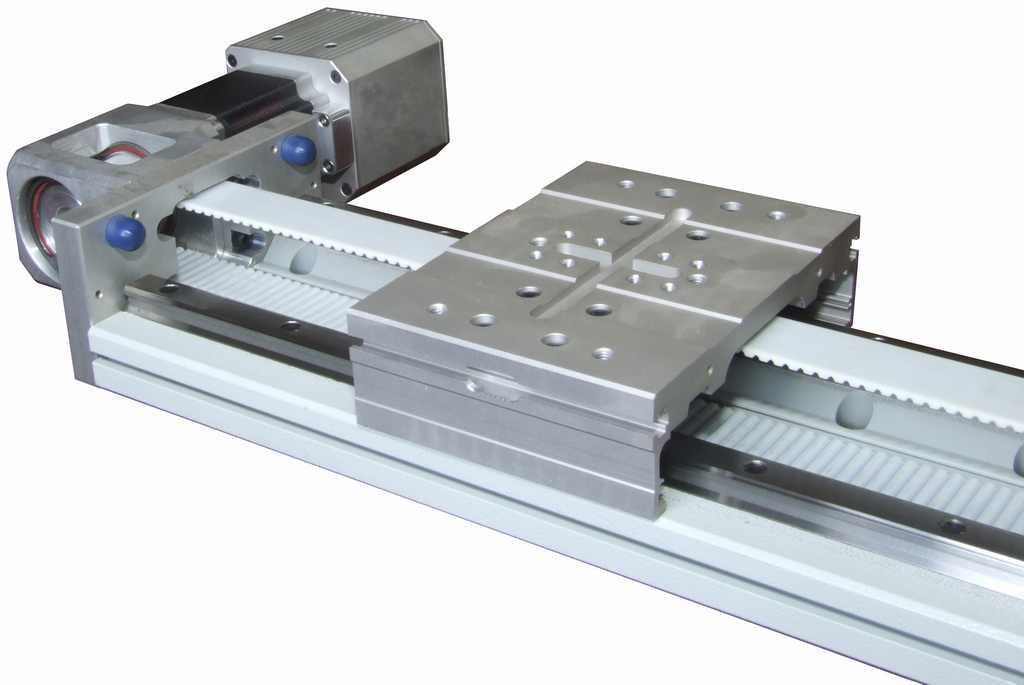
\includegraphics[width=0.7\textwidth]{ch-2/image19}
	}
	\caption{Линейный привод на основе зубчатого ремня.}\label{fig:belt}
\end{figure}

Линейные приводы на основе зубчатых ремней нашли широкое применение в современном высокоточном оборудовании, однако было принято решение не использовать ее при проектировании линейных приводов УШ. Данное решение обосновано необходимостью создания не просто надежного и универсального механизма перемещения потального типа, но и желанием добиться избыточности по некоторым параметрам, например, получить привод с максимально возможной нагрузочной способностью без увеличения габаритов и сложности конструкции. По этой причине предпочтение было отдано винтовой передаче. При этом зубчатый ремень тоже будет использован, но только как вспомогательный механизм (о чем будет сказано далее в этом разделе).

Перейдем к рассмотрению винтовых передач, а точнее шариково-винтовых пар~(рисунок~\cref{fig:ballscrew}), так как именно этот тип является наиболее распространенным на сегодняшний день\footnote{Передачи скольжения (<<ласточкин хвост>>) и роликово-винтовые передачи не рассматривались в силу их избыточности.}.

Шариково-винтовая пара является разновидностью передачи качения, в которой промежуточными телами являются закаленные шарики. Конструктивно шариково-винтовая пара состоит из винта и гайки с~канавками специального профиля. Шарики движутся по замкнутой траектории, проходящей через канавки винта и витки гайки через перепускные каналы (возвратные трубки), находящиеся в специальных вкладышах, расположенных в окне гайки.

Парные витки гайки продольно смещены по отношению к канавкам винта в двух направлениях, что обеспечивает преднатяг механизма и~компенсацию возможного люфта~(рисунок~\cref{fig:ballscrew-1}). Также в конструкции шариково-винтовой пары предусмотрены лубрикаторы, обеспечивающие постоянную смазку механизма густой смазкой, и грязесъемные кольца.

\begin{figure}[ht]
	\centerfloat{
		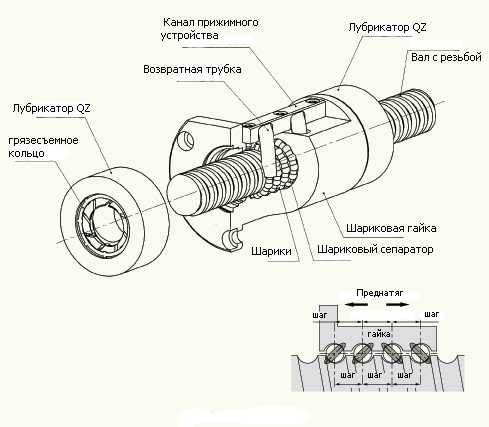
\includegraphics[width=0.7\textwidth]{ch-2/image20}
	}
	\caption{Конструкция шарико-винтовой пары.}\label{fig:ballscrew}
\end{figure}

\begin{figure}[ht]
	\centerfloat{
		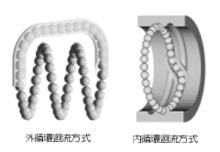
\includegraphics[width=0.7\textwidth]{ch-2/image21}
	}
	\caption{Схема движения тел качения в шариково-винтовой паре.}\label{fig:ballscrew-1}
\end{figure}

Основные достоинства шарико-винтовой пары:

\begin{itemize}
	\item Высокий КПД, определяющийся малыми потерями на трение.
	\item Большая нагрузочная способность при достаточно малых габаритах.
	\item Высокая точность перемещения, обусловленная практически полным отсутствием люфта.
	\item Самоторможение механизма при выходе из строя двигателя привода.
	\item Высокое быстродействие, определяемое значительной скоростью вращения винта.
	\item Плавный ход и бесшумность.
\end{itemize}

Из выявленных недостатков можно выделить следующие:

\begin{itemize}
	\item Сложность конструкции гайки.
	\item Достаточно высокая в сравнении с передачей на зубчатом ремне цена.
\end{itemize}

Тем не менее, именно конструкция линейного привода на основе шариково-винтовой пары признана наиболее оптимальной и~удовлетворяющей основным требованиям к УШ. 

Последний этап проектирования линейного привода "--- выбор двигателя. Выбор делался между двумя типами вращающихся двигателей: шаговых и серводвигателей. Данные типы имеют принципиальные конструктивные отличия. Шаговый двигатель является синхронным бесколлекторным двигателем с несколькими парными обмотками, расположенными в статоре~(рисунок~\cref{fig:stepper}). Подача тока на одну из обмоток приводит к изменению положения ротора (его фиксацию по отношению к~одному из полюсов многополюсного постоянного магнита ротора). Циклическая активация (переключение) обмоток вызывает дискретные угловые перемещения ротора, именуемые шагами.

\begin{figure}[ht]
	\centerfloat{
		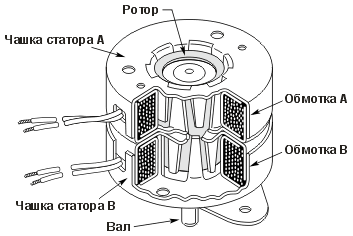
\includegraphics[width=0.7\textwidth]{ch-2/image22}
	}
	\caption{Конструкция шагового двигателя.}\label{fig:stepper}
\end{figure}

Серводвигатель~(рисунок~\cref{fig:servo}) представляет собой обычный электрический двигатель (как правило, постоянного тока, снабженный понижающим зубчатым редуктором или без него, в зависимости от требований к создаваемому моменту на валу двигателя) с обязательной схемой управления с отрицательной обратной связью по положению вала. Для обеспечения обратной связи используются датчики угла поворота различных конструкций, начиная с простейших потенциометров и~заканчивая прецизионными оптическими или магнитными энкодерами.

Перейдем к рассмотрению достоинств и недостатков двигателей обоих типов. Основными достоинствами \textit{серводвигателей} являются:

\begin{itemize}
	\item В случае использования механического редуктора серводвигатель может создавать достаточно большое для своих габаритов и массы усилие на валу.
	\item Точность позиционирования серводвигателя определяется типом используемого датчика углового положения и может быть достаточно высокой.
	\item Высокий КПД, достигающий 90\% при малых нагрузках.
	\item Низкая инертность и способность к очень быстрому ускорению даже при высокой нагрузке.	
\end{itemize}

\begin{figure}[ht]
	\centerfloat{
		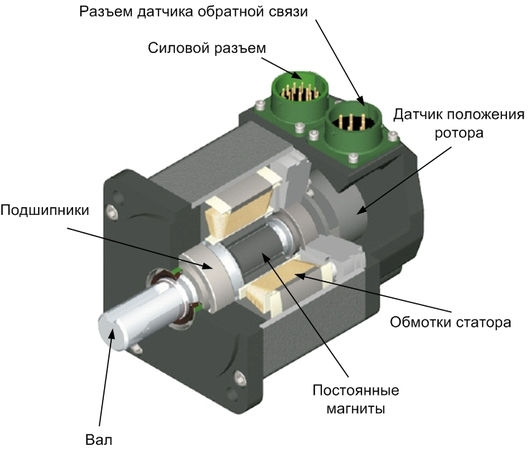
\includegraphics[width=0.7\textwidth]{ch-2/image23}
	}
	\caption{Конструкция безредукторного серводвигателя, созданного на основе трехфазного бесколлекторного двигателя постоянного тока.}\label{fig:servo}
\end{figure}

\begin{itemize}
	\item Низкая рабочая температура, так как ток потребляется пропорционально нагрузке.
	\item Пиковая мощность и крутящий момент могут быть в несколько раз больше номинальных, что позволяет использовать серводвигатели в жестких условиях эксплуатации (естественно, если будет создана система экстренного охлаждения).
	\item Серводвигатели работают плавно и практически бесУШмно даже на больших скоростях.
	\item Серводвигатели не подвержены влиянию резонанса и~вибрации на всем диапазоне рабочих частот.
\end{itemize}

К недостаткам серводвигателей можно отнести:

\begin{itemize}
	\item Мощные серводвигатели требуют создания воздушной системы охлаждения, вентиляционные каналы которой могут засоряться в процессе работы.
	\item Максимальный момент серводвигатели отдают на очень высоких оборотах, поэтому как правила должны изготавливаться в сборе с редуктором.
	\item Требуют достаточно мощных и защищенных от кратковременных перегрузок источников питания.
	\item В случае заклинивания механизма или длительной перегрузке серводвигатель можно быстро перегореть. Единственный способ борьбы с этим явлением использование дополнительных датчиков нагрузки и специальной программы управления не допускающей длительных перегрузок.
	\item Сложный алгоритм управления, который требует использования дорогостоящих контроллеров, энкодеров и~предварительной калибровки и настройки, так как основной алгоритм управления данным типом двигателя предполагает создания пропорционально-интегрально-дифференциального регулятора.
	\item Более высокая по сравнению с шаговыми двигателями стоимость, обусловленная необходимостью использования дорогостоящих редукторов, энкодеров и схем регулирования и~управления.
\end{itemize}

Достоинствами \textit{шаговых двигателей} являются:

\begin{itemize}
	\item Высокая точность и стабильность шага, не зависящая от приложенной нагрузки.
	
	\item Не требует наличия обратных связей по положению, так как имеет фиксированный угол поворота.
	
	\item Шаговые двигатели являются очень распространенными и~производятся повсеместно, что определяет их невысокую стоимость. В случае поломки его можно просто заменить.
	
	\item Более долгий по сравнению с серводвигателями срок эксплуатации.
	
	\item Более простая система управления. Существует огромное количество готовых интегральных драйверов, сочетающих в~себе силовую часть и блок управления, которому нужен только тактовый сигнал от микроконтроллера. В простейшем случае можно обойтись только силовой частью, а~последовательность шагов генерировать с помощью микроконтроллера.
	
	\item В случае превышения максимальной нагрузки двигатель не сгорает, так как работа в режиме удержания является для него штатным режимом.
	
	\item Обеспечивает достаточный крутящий момент даже на низких оборотах, что не требует применения редукторов.
	
	\item Отличная повторяемость, как правило, в штатном режиме шаговый двигатель не должен пропускать шаги.	
\end{itemize}

Недостатки шаговых двигателей следующие:

\begin{itemize}
	\item Высокое энергопотребление, не зависящее от нагрузки.
	
	\item Пропорциональное снижение крутящего момента с~повышением оборотов.
	
	\item Низкая точность, обусловленная тем, что шаг задается полюсами постоянного магнита ротора, количество, которых по понятным причинам не может быть очень большим. Стандартное количество шагов для большинства шаговых двигателей 200 или 400. Низкая точно частично может быть скомпенсирована использованием микрошагового режима, который реализуется в блоке управления и позволяет ротору находиться в промежуточном положении между полюсами, а~также возможностью применения внешних съемных редукторов, которые лишь немного увеличивают габариты шагового двигателя.
	
	\item Возможно появление резонанса, что опять же может быть скомпенсировано применением микрошага.
	
	\item Полное отсутствие контроля положения вала.
	
	\item Даже в штатном режиме шаговый двигатель ощутимо нагревается, однако конструкция шагового двигателя позволяет эффективно рассеивать это тепло, система принудительно охлаждения, как правило, не требуется.
	
	\item Под нагрузкой не может начать движение сразу на высокой скорости. Требуется реализация плавного разгона и~торможения.
	
	\item Не может мгновенно восстанавливаться после перегрузки.
	
	\item Значительно УШмит на средних и высоких скоростях, что также частично компенсируется использованием микрошага.
	
	\item Для своих габаритов и массы имеет недостаточную по сравнению с серводвигателями мощность.
\end{itemize}

Анализ показал, что оба типа двигателей удовлетворяют всем требованиям, предъявляемым к УШ. Поэтому было найдено следующие компромиссное решение: основные линейные приводы координатного стола (обеспечивающие перемещение по координатам X и Y), а также линейный привод опциональной координаты Z приводятся в движение шаговыми двигателями без редукторов с количеством шагов, равном 400 (максимальное количество шагов для двигателей данного типа).

При этом на осях предусматривается крепление для вращающихся оптических инкрементальных энкодеров, контролирующих положение шариково-винтовых пар и не допускающих пропуск шагов. Разрешающая способность энкодеров должна быть в несколько раз выше количества шагов.

Для обеспечения плавности хода и снижения явления вибрации предполагается применение недорого интегрального драйвера с~возможностью генерации микрошага (16--32 микрошага). Повышение точности позиционирования за счет использования микрошага не предполагается, программа управления работает только с целыми шагами, опираясь на показания датчиков положения. Компенсация погрешности позиционирования задается реализацией простейшего пропорционального регулятора.

\subsection{Итоговая схема компоновки координатного стола универсального шасси}

На рисунке~\cref{fig:scheme} представлена итоговая Электрокинематическая схема координатного стола УШ. Перемещение рабочего органа по оси Y осуществляется за счет поперечной опорной траверсы, перемещающейся по направляющим 10. Направляющие выполнены из закаленного круглого прутка с опорой, поперечная балка опирается на ползуны с линейными подшипниками 5.

Для предотвращения заклинивания поперечной балки при движении по направляющим применена классическая схема, с размещение с одной стороны балки двух разнесенных по отношению друг к другу подшипников, а с другой "--- одного. Ползуны соединены с гайкой шариково-винтовой пары 7, опирающейся с двух сторон на радиальные подшипники 4 и 6. Шариково-винтовая пара располагается непосредственно над опорной направляющей и является полностью разгруженной, то есть не испытывает никаких радиальных нагрузок. На поперечной балке также размещена цилиндрическая направляющая и шариково-винтовая пара оси X.

\begin{figure}[ht]
	\centerfloat{
		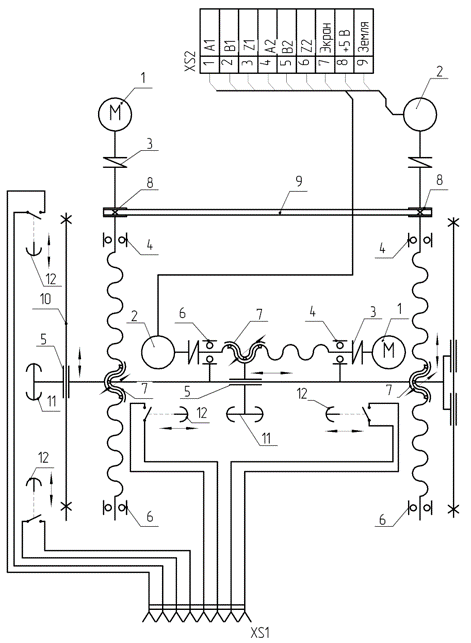
\includegraphics[width=0.7\textwidth]{ch-4/el-mech-sch}
	}
	\caption[Электрокинематическая схема координатного стола УШ]{Электрокинематическая схема координатного стола УШ: 1 "--- двигатель шаговый, 2 "--- датчик угла поворота, 3 "--- муфта кулачковая, 4 "--- Подшипник радиальный, 5 "--- подшипник линейный, 6 "--- Подшипник радиальный, 7 "--- ШВП, 8 "--- Шкив зубчатый, 9 "--- Ремень зубчатый, 10 "--- Направляющая, 11 "--- Щелевой оптический датчик, 12 "--- Выключатель концевой}\label{fig:scheme}
\end{figure}


Ползун оси X соединен с плоскостью универсального крепления рабочего органа или сменного модуля.

Вращение шарико-винтовых пар осуществляется с помощью шагового двигателя 1 форм-фактора NEMA23 с квадратным фланцем со стороной 57 мм (экспериментальный образец создан на основе китайских двигателей FL57STH76-3005MA с разрешением 400 шагов на оборот). Сопряжение двигателя с шарико-винтовой пары достигается за счет кулачковой муфты 3. Синхронизация валов обеспечивается зубчатым ремнем 9 и зубчатыми шкивами 8, также предусмотрена система натяжения ремня, представляющая собой свободно вращающийся шкив и пружину сжатия.

Обратная связь по положение достигается использованием вращающихся инкрементальных энкодеров 2 (предполагается использование отечественных датчиков, например, ЛИР-158).

Энкодеры сопрягаются с шариково-винтовой парой путем использования кулачковых муфт. Для оси Y датчик крепится не на основной шариково-винтовой паре, а на вспомогательной, синхронизированной через зубчатый ремень. Таким образом, отсутствует необходимость использования отдельного датчика обрыва ремня. 

Каждая ось УШ снабжена двумя механическими концевыми выключателями 12. Функция концевых выключателей "--- экстренный останов ползуна при достижении края направляющей для предотвращения поломок от их соударения. Концевые выключатели подключены в обход основной схемы управления и не зависят от основного управляющего контроллера. Система экстренной остановки будет работать даже в случае зависания или выхода из строя основного микроконтроллера управления. Последнее достигается за счет использования простой логической схемы, которая при замыкании любого из двух концевых выключателей оси переводит шаговый двигатель в режим удержания (питание подается на обе фазы одновременно, благодаря чему происходит магнитное торможение двигателя). В конструкции также предусмотрены концевые противоударные элементы, выполненные в виде резиновых, пружинных или тросовых гасителей.

На обоих ползунах размещены щелевые оптически датчики 11, необходимые для самокалибрования УШ. Предполагается, что каждый раз при включении установки ползуны обеих осей будут на минимальной скорости перемещаться в одном направлении до срабатывания первого оптического датчика, а затем в противоположном до второго. При этом энкодер зафиксирует, сколько шагов можно будет сделать по каждой из осей, зафиксировав тем самым нулевую и максимальную координату каждой из осей. Данный подход позволяет компенсировать любые деформации механизма, возникающие, например, из-за перепада температуры.

\section{Универсальный блок управления и программное обеспечение}

\subsection{Универсальный блок управления УШ}

УШ является центральным компонентом МТП, так как позволяет связать аппаратную часть создаваемого на базе этой концепции оборудования (занимается получением данных от датчиков УШ и рабочих органов, генерирует управляющие сигналы приводов) и программную часть (связывает оборудование с ПК и позволяет осуществлять двухсторонний обмен данными с МТП). Универсальный блок управления состоит из следующих модулей:

\begin{itemize}
	\item Модуль питания.
	\item Процессорный модуль.
	\item Модуль сопряжения с ПК.
	\item Модуль сопряжения с датчиками.
	\item Модули управления приводами.
	\item Модуль индикации и взаимодействия с оператором.
\end{itemize}

Все модули будут снабжены собственным микроконтроллером, обеспечивающим их взаимодействие по протоколу \foreignlanguage{english}{SPI}\footnote{сокр.~от~англ. англ. \textit{Serial Peripheral Interface, SPI bus} "--- последовательный периферийный интерфейс, шина SPI.} Данный протокол позволит всем модулям соединяться между собой и обмениваться необходимой информацией в синхронном последовательном режиме. То есть универсальный блок управления будет представлять собой сеть микроконтроллеров, обеспечивающих различные функции.

В качестве \textit{модуля питания} предполагается взять стандартный промышленный блок питания, работающий на напряжении~\SI{48}{\volt} постоянного тока и обеспечивающий мощность порядка~\SIrange{400}{500}{\watt}.

Для получения различных напряжений, необходимых, например, для питания микроконтроллера, датчиков, двигателей, энкодеров и~др. предполагается создание сменных плат питания, построенных на базе современных импульсных стабилизаторов напряжения с высоким КПД таких, как LM2940, LT1185, LT1528 и~др. Подобные регуляторы могут обеспечивать ток до~\SI{3}{\ampere} (возможно запараллеливание для достижения больших значений тока), требуют минимальной обвязки и очень дешевы, выходное напряжение в них задается подстроечным резистором, который после настройки каждой платы должен быть опломбирован.

\textit{Процессорный модуль} будет выполнять функции по управлению УШ, получению и обработке данных, полученных от других модулей, а также вспомогательные функции, например, индикация и взаимодействие с оператором.

Наиболее важная функция программного обеспечения универсального блока управления "--- получение и обработка G-кодов, полученных от ПК (интеграция с \foreignlanguage{english}{МПО}).

Модуль будет построен на базе тридцатидвухбитного процессора семейства \foreignlanguage{english}{ARM}. Выбор обусловлен имеющимся положительным опытом работы с микроконтроллерами этого семейства архитектур, в частности, использовались контроллеры \foreignlanguage{english}{STMicroelectronics}, \foreignlanguage{english}{Texas Instruments}, \foreignlanguage{english}{NXP} и~др. Для данного проекта предполагается использование отечественных микроконтроллеров, производимых ЗАО~<<ПКК Миландр>>.

\textit{Модуль сопряжения с ПК} необходим для взаимодействия с исполнительными устройствами и датчиками оборудования, построенного на базе концепции \foreignlanguage{english}{МТП}. Предполагается, что обмен данными между универсальным блоком управления будет осуществляться через стек протоколов \foreignlanguage{english}{TCP/IP}\footnote{сокр.~от~англ. \textit{Transmission Control Protocol/Internet Protocol} "--- протокол передачи данных/интернет-протокол.}, на прикладном уровне будет использован протокол \foreignlanguage{english}{HTTPS}\footnote{сокр.~от~англ. \textit{HyperText Transfer Protocol Secure} "--- защищенный протокол передачи гипертекста.} с самоподписанным сертификатом; на канальном "--- возможно использование протоколов \foreignlanguage{english}{Ethernet} (для проводного соединения) и IEEE 802.11 Wireless Ethernet (для беспроводного). Подобная реализация позволит легко интегрировать оборудование, построенное в соответствие с концепцией \foreignlanguage{english}{МТП} в существующую локальную сеть (включая возможность доступа через Интернет), а также позволит работать с ним без установки каких-либо драйверов или другого вспомогательного программного обеспечения. Программная реализация данного взаимодействия будет рассмотрена в следующем разделе.

\textit{Модуль сопряжения с датчиками} будет обрабатывать информацию, полученную от датчиков. Предполагается, что большинство современных датчиков являются либо аналоговыми, либо цифровыми и работают по одному из протоколов взаимодействия: \foreignlanguage{english}{SPI}, \foreignlanguage{english}{I}2\foreignlanguage{english}{C}, 1-\foreignlanguage{english}{Wire}, \foreignlanguage{english}{CAN} (сокр.~от~англ. \textit{Controller Area Network} "--- сеть контроллеров).

В случае использования аналоговых датчиков, сигнал должен быть усилен с~помощью операционного усилителя и оцифрован посредством аналогово-цифрового преобразователя (сокр. \textit{АЦП}). Оба этих компонента имеют возможность программного управления, то есть необходимость усиления сигнала, разрядность АЦП и другие параметры могут быть заданы отдельно для каждого аналогового датчика.

Если же сигнал цифровой, необходимо согласование протокола, по которому работает датчик и внутреннего протокола универсального блока управления "--- \foreignlanguage{english}{SPI}. Согласование осуществляется программно на этапе первичной настройки универсального блока управления под конкретный тип оборудования.

Дополнительно модуль сопряжения с датчиками будет включать в~себя подмодуль преобразования логических уровней, так как возможно несовпадение напряжения питания какого-либо датчика с основным логическим напряжением универсального блока управления (для процессоров семейства \foreignlanguage{english}{ARM}, как правило, логические уровни задаются напряжением от 0 до 3,3~В).

\textit{Модули управления приводами} являются силовыми и позволяют управлять шаговыми двигателями и прочими электродвигателями, используемыми в оборудовании, создаваемом на базе концепции \foreignlanguage{english}{МТП}. Например, для управления шаговыми двигателями, модули могут быть построены на базе популярных интегральных драйверов шаговых двигателей, например, \foreignlanguage{english}{L}297+\foreignlanguage{english}{L}298, \foreignlanguage{english}{DRV}8825 или \foreignlanguage{english}{TB}6600. В~зависимости от задач, решаемых конкретным типом оборудования, возможно использование и более сложные и дорогие схемы управления двигателями, при этом универсальность достигается единым протоколом взаимодействия с процессорным модулем. Предполагается, что процессорный модуль при необходимости будет взаимодействовать с 8 модулями управления приводами.

\textit{Модуль индикации и взаимодействия с оператором} позволяет отображать важную информацию о текущем состоянии оборудования с~помощью различных типов индикаторов (сегментных, жидкокристаллических и~др.), а также взаимодействовать с оператором без подключения к ПК.

Данный модуль необходим для первичной настройки оборудования (например, присвоения внутреннего адреса в локальной сети, к которой оно будет подключено или параметров беспроводной точки доступа), восстановления после сбоев и прочих операций, которые невозможно или нецелесообразно производить через основной интерфейс управления. Данный модуль является опциональным и все его функции должны быть продублированы в основном интерфейсе взаимодействия с оборудованием, реализуемым на ПК.

\begin{figure}[ht]
	\centerfloat{
		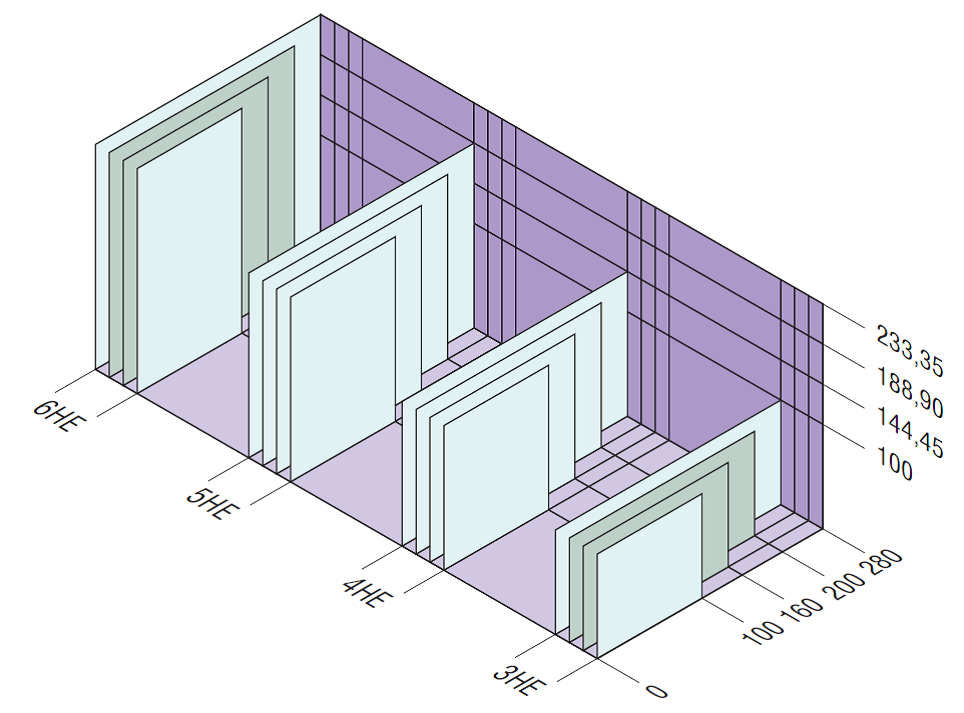
\includegraphics[width=0.7\textwidth]{ch-2/image26}
	}
	\caption{стандартные типоразмеры печатных плат модулей универсального блока управления.}\label{fig:euromech}
\end{figure}

Конструктивно все модули должны быть выполнены по стандарту МЭК 60297 (известному как <<Евромеханика>>), то есть с возможностью размещения в стандартных корзинах девятнадцатидюймовых телекоммуникационных стоек. Типоразмеры печатных плат, удовлетворяющих данному стандарту, представлены на рисунке~\cref{fig:euromech} (\foreignlanguage{english}{HE} "--- единица, в которой задаётся ширина конструкции, равна 5,08 мм (0,2 дюйма), длины плат задаются в миллиметрах).

На задней стенке корзин будут располагаться разъёмы подключения модулей, а на задней части модуля ответная часть разъёма. Установка модуля приводит к совмещению разъёмов. Будут использованы разъёмы типа DIN 41612 или СНП-59.


\section{Выводы по главе 4}

Были рассмотрены вопросы создания универсальной платформы технологического оборудования МТП. Данная платформа является программно-аппаратным комплексом, позволяющим за счет унификации и параметризации своих составных частей создавать различные виды оборудования с числовым программным управлением.

Основная область применения подобных устройств "--- малые инновационные предприятия. Данные структуры, как правило, занимаются проектированием и единичным или мелкосерийным производством высокотехнологичного оборудования и поэтому нуждаются в собственной производственной базе.

Концепция МТП позволит малым инновационным предприятиям иметь универсальную платформу, на базе которой они самостоятельно (или с привлечением сторонних специалистов) смогут создавать все необходимое для них оборудование не только для производства готовых изделий, но и для проведения всего комплекса исследований, связанных с этим процессом.

В рамках концепции предполагается разработка трехкоординатного шасси портальной конструкции, универсального блока управления, состоящего из набора взаимозаменяемых модулей с общим интерфейсом взаимодействия, модульного программного обеспечения с открытым исходным кодом, позволяющего расширять и модернизировать свой функционал за счет написания или добавления новых модулей, а также набора требований для проектирования рабочих органов, определяющих основное назначение оборудования, создаваемого на базе концепции.


\FloatBarrier

%\nocite{*}

\FloatBarrier